\documentclass[a4paper, 12pt]{article}
\usepackage{graphicx}
\usepackage{listings}
\usepackage{tikz}
\usepackage{amssymb}
\usepackage{dot2texi}
\usetikzlibrary{automata, positioning, arrows}
\usepackage{booktabs}
\usepackage{tablefootnote}
\usepackage{adjustbox}
\usepackage{caption}
\usepackage{subcaption}


\setlength\parindent{24pt}

\lstset{language=python,breaklines=true, frame=single}
\tikzset{
        ->,  % makes the edges directed
        %>=stealth’, % makes the arrow heads bold
        node distance=6cm, % specifies the minimum distance between two nodes. Change if n
        every state/.style={thick, fill=gray!10}, % sets the properties for each ’state’ n
        initial text=$ $, % sets the text that appears on the start arrow
        }

\begin{document}
\begin{figure}
    \centering
    
\includegraphics[width=1\textwidth]{Logo}
\end{figure}

\title{CPS3233 Assignment Report}
\author{Manwel Bugeja}
\date{\today}
\maketitle
  
\tableofcontents
\newpage

\section{Elevator System Specification}
In this section, the specifications of the elevator system are expressed in several different formal notations. The notations are Finite State Automata (FSAs), Regular Expressions (RE), Timed Automata (TAs) and Duration Calculus (DC). From the ones listed, TAs and DC are the capable of expressing timed events. \\

\subsection{Finite State Automata}
A finite state automata was designed to describe the elevator system. The formal definition of the state machine can be seen in listing \ref{lst:FSA}. The lift can be in one of three states: Idle, Loading or Moving. Idle is when the lift is not moving and has its door closed. Loading when the lift is not moving but has the doors open. Moving is when the lift is moving either up or down. Note that a 'bad' state could be added for when the lift is moving and has the doors open as the lift should never be in this state. \\

This FSA describes the flow of the lift lifetime in a very basic nature for example it does not consider elevator summoning or floor requests. This can be seen visually in figure \ref{fig:FSA}. A more detailed automaton considering more actions and time constraints is discussed in section \ref{sec:timed-automata}.



\begin{lstlisting}[
caption={FSA definition}
\label{lst:FSA}
]
M = {
{Idle, Loading, Moving},
{openDoor, closeDoor, stop, goUp, goDown},
{
    Idle, openDoor -> Loading,
    Idle, goUp -> Moving,
    Idle, goDown -> Moving,
    Loading, closeDoor -> Idle,
    Moving, stop -> Idle
},
Idle,
{}
}
\end{lstlisting}





\begin{figure} % ’ht’ tells LaTeX to place the figure ’here’ or at the top of the page
    \centering % centers the figure
    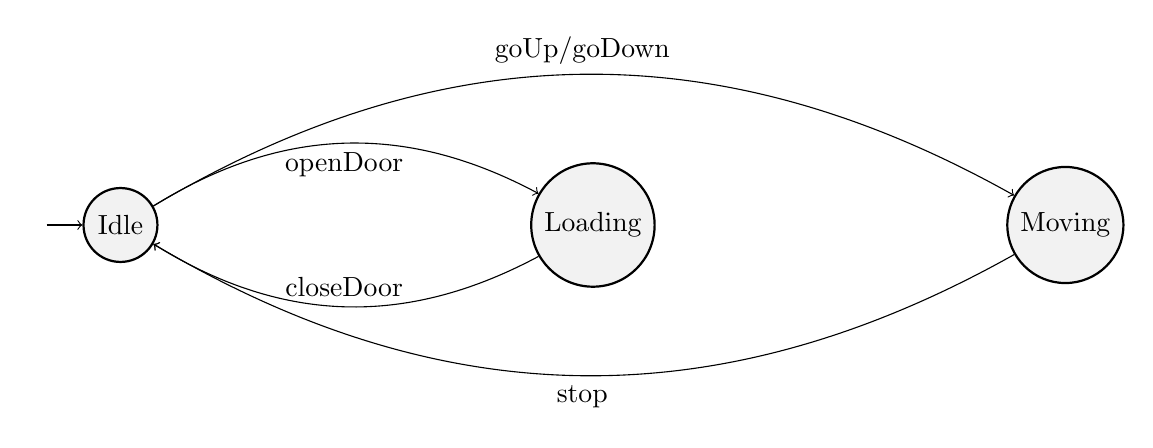
\begin{tikzpicture}
        % tikz code goes here
        \node[state, initial] (Idle) {Idle};
        \node[state, right of=Idle] (Loading) {Loading};
        \node[state, right of=Loading] (Moving) {Moving};
        
        \draw (Idle) edge[bend left, below] node{openDoor} (Loading);
        \draw (Loading) edge[bend left, above] node{closeDoor} (Idle);
       	\draw (Idle) edge[bend left, above] node{goUp/goDown} (Moving);
	\draw (Moving) edge[bend left, below] node{stop} (Idle);
        
    \end{tikzpicture}
    \caption{Basic FSA}
    \label{fig:FSA}
\end{figure}


\subsection{Regular Expressions}
The lift system was also expressed via regular expressions. This RE can be seen in listing \ref{lst:RE}. The RE starts of with a series of \textit{openDoor} and \textit{closeDoor} actions which must occur consecutively. This is done so that when the lift moves to the next stage in the RE, the door is always closed, since the lift cannot move with its door open. \\

Next, the RE verifiers that the lift goes an arbitrary number of steps up or down (depending on what the user decided) followed by a stop. The \textit{stop} is there to make sure the lift is not moving when the progress move back to the open/close door part of the expression. \\

An example run of the elevator is:
\texttt{openDoor > closeDoor > goUp > goUp > stop > openDoor > closeDoor > openDoor > closeDoor > goDown > stop}.
This run through is correct according to the RE provided. 

\begin{lstlisting}[
caption={RE definition}
\label{lst:RE}
]
((openDoor.closeDoor)* (goUp* + goDown*).stop )*

\end{lstlisting}


\subsection{Timed Automata}
\label{sec:timed-automata}
For the timed automata (figure \ref{fig:TA}, the same state machine above was used with some clocks and states added to verify time-constrained events. In the formal definition of the automaton, the transition functions where modified to accommodate such changes. The formal specification can be seen in listing \ref{lst:TA}. The transition functions follow the format \texttt{[from, to, letter, clocks reseted, condition]}. \\

The first time property that is handled says that "upon a request, after the door closes, the elevator starts moving in less than 3 seconds". When adapted to the provided automaton, this translates to "when the lift is \textit{Idle} (because a floor button was pressed so the door closed), it goes either up or down in less than 3 seconds". This is verified by clock x. \\

The second time property expresses that "after the door has been open for 3 seconds, it closes automatically". This implies that when the lift has its doors opened i.e. its in the \textit{Loading} state, it must go to the \textit{Idle} in less than 3 seconds. This is because if a user presses the button in less than 3 seconds, the door will close and if he does not press any button, the door closes automatically. This is verified by clock y.  \\

The two new states are \texttt{Requested} and \texttt{LoadingRequested}. A new event, \texttt{requested} is also added to the alphabet. These new additions concern the summon button present at each floor. The \texttt{Requested} state signifies when the lift a floor was requested while the lift was moving or idle. The state \texttt{LoadingRequested} is the same except that before the request, the lift was in the \texttt{Loading} state. \\

The state \texttt{Requested} was added for the time property that states that the lift must start moving in less than 3 seconds i.e., the time property handles by clock x. Therefore, every transition that leads to the \texttt{Requested} state resets clock x. Meanwhile, \texttt{LoadingRequested}) is needed for the close-door time property handled by clock y. 

\begin{lstlisting}[
caption={TA definition}
\label{lst:TA}
]
M = {
{openDoor, closeDoor, stop, goUp, goDown},
{Idle, Loading, Moving},
{idle},
{x, y},
{
    [ Idle, Loading, openDoor, {y:=0}, true ]
    
    [ Idle, Requested, request, {x:=0}, true ]
        
    [ Loading, Idle, closeDoor, {x:=0}, y<3 ]
    
    [Loading, LoadingRequested, request, {}, true]
    
    [ Moving, Idle, stop, {x:=0}, true ]
    
    [ LoadingRequested, Requested, closeDoor, {x:=0}, y<3 ]
    
    [ Requested, Moving, goUp/goDown, {}, x<3 ]
}
}
\end{lstlisting}


\begin{figure}%  figure placement: here, top, bottom, or page
   \centering
\begin{adjustbox}{max width=\textwidth}


    \centering % centers the figure
    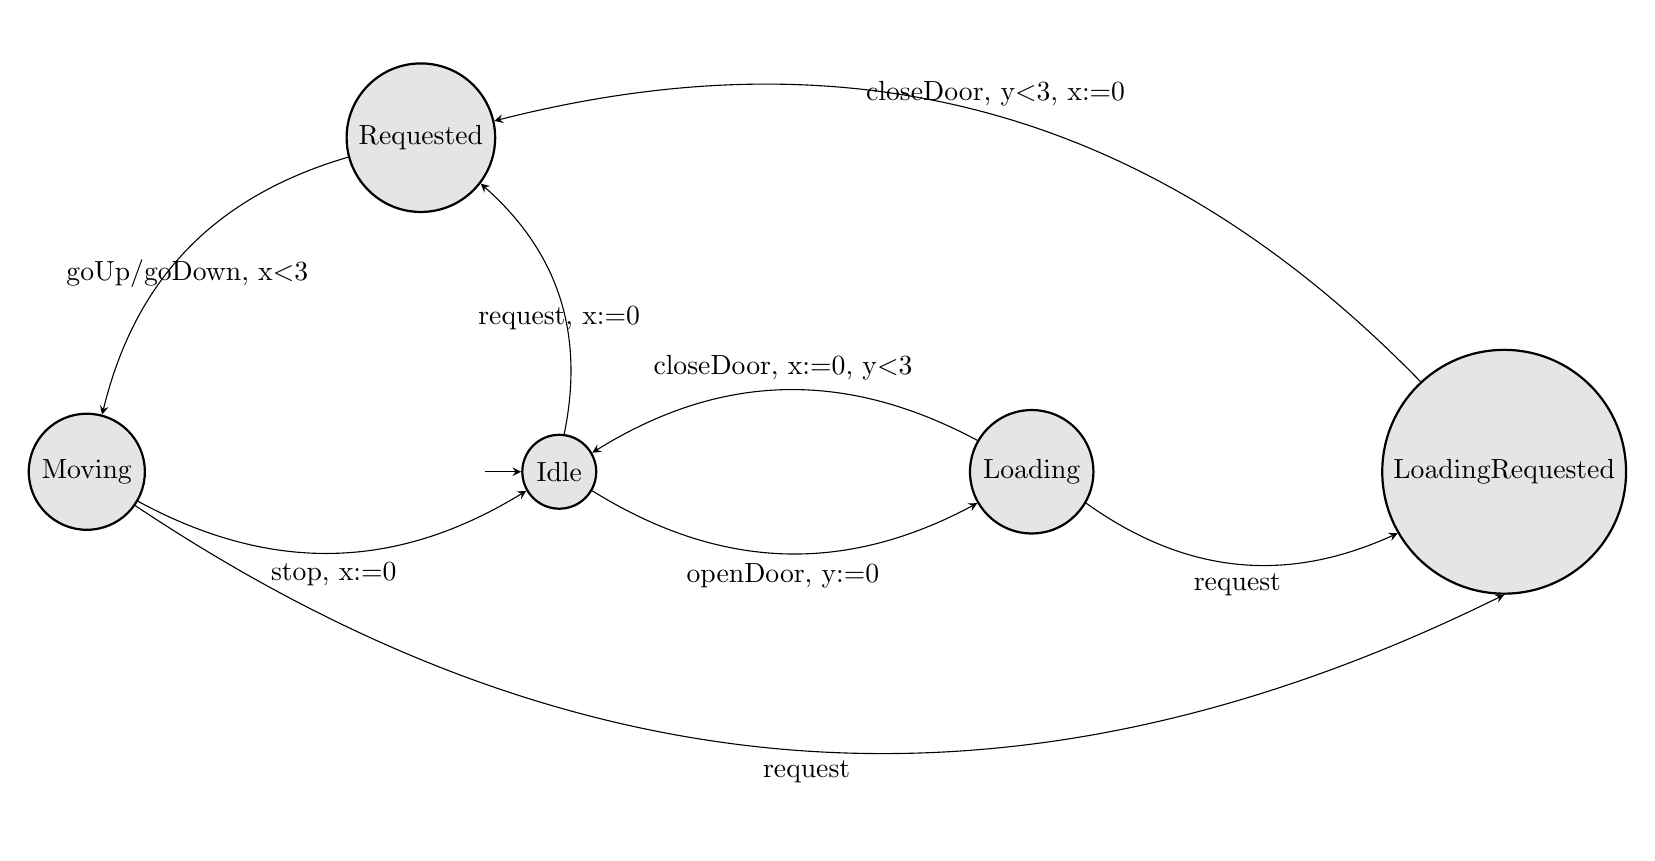
\begin{tikzpicture}[>=stealth,auto,state/.append style={fill=black!10}]
        % tikz code goes here
        \node[state, initial] (Idle) {Idle};
        \node[state, right of=Idle] (Loading) {Loading};
        \node[state, left of=Idle] (Moving) {Moving};
        \node[state, above right of=Moving] (Requested) {Requested};
        \node[state, right of=Loading] (LoadingRequested) {LoadingRequested};
        
        \draw (Idle) edge[bend right, below] node{openDoor, y:=0} (Loading);
        \draw (Loading) edge[bend right, above] node{closeDoor, x:=0, y$<$3} (Idle);
	\draw (Moving) edge[bend right, below] node{stop, x:=0} (Idle);
	\draw (Moving) edge[bend right, below] node{request} (LoadingRequested.south);
	\draw (Requested) edge[bend right, below] node{goUp/goDown, x$<$3} (Moving);
	\draw (Loading) edge[bend right, below] node{request} (LoadingRequested);
        \draw (LoadingRequested) edge[bend right, above] node{closeDoor, y$<$3, x:=0}(Requested);
        \draw (Idle) edge[bend right, below] node{request, x:=0} (Requested);
        
    \end{tikzpicture}

\end{adjustbox}

\caption{TA figure}
\label{fig:TA}

\end{figure}




\subsection{Duration Calculus}
For the DC specifications, two formulas where defined, one for each time constrain. The first time constrain states that: "upon a request, after the door closes, the elevator starts moving in less than 3 seconds". This is expressed by the formula:

$$\square [Idle] ; [Loading] ;  [Moving]  \wedge [idle] ; [Loading] ; [Idle] \Rightarrow \int loading < 3$$

The square means that it is checking for all subintervals. Then the pattern the formula is looking for is \textit{Idle}, followed my \textit{Loading}, followed by \textit{Moving}. Then, the expression verifies that the time of loading is less than 3.

The second time constrain says that: after the door has been open for 3 seconds, it closes automatically". The formula describing this is as follows:

$$\square [doorOpen] ; [\neg doorOpen] \Rightarrow \int doorOpen < 3$$

The formula looks for the pattern of an open door followed by a closed door and then verifies that the door was open for less than 3 seconds. 

\section{Runtime Verification}

For runtime verification (RV), the Larva tool was used. The automata applied where directly derived from the automata discussed in section \ref{sec:timed-automata}. However, it was not implemented as a single automaton in order to check for properties individually. On top of that, several bas states where added since the ones shown do not include them to make it visually easier. The full automata including the bad states where generated and can be seen later on. \\

The first property investigated was the door close property (seen visually in figure \ref{fig:generated-automaton-LiftOpenTimeProperty}) . First off, to make the investigation simpler, a single lift was considered. This is because the automaton designed only considers one lift. The Java code was analysed to find the methods that correspond with the designed events. These methods were present in \textit{Lift.java}. The methods and their corresponding events is shown in table \ref{tab:lift-open-time-property}. \\

This property does not only check for the time property. It also checks for temporal properties such as receiving a \texttt{openDoor} signal while already open. It also checks for lift movement while the lift is open. 

\begin{figure}
   \centering
   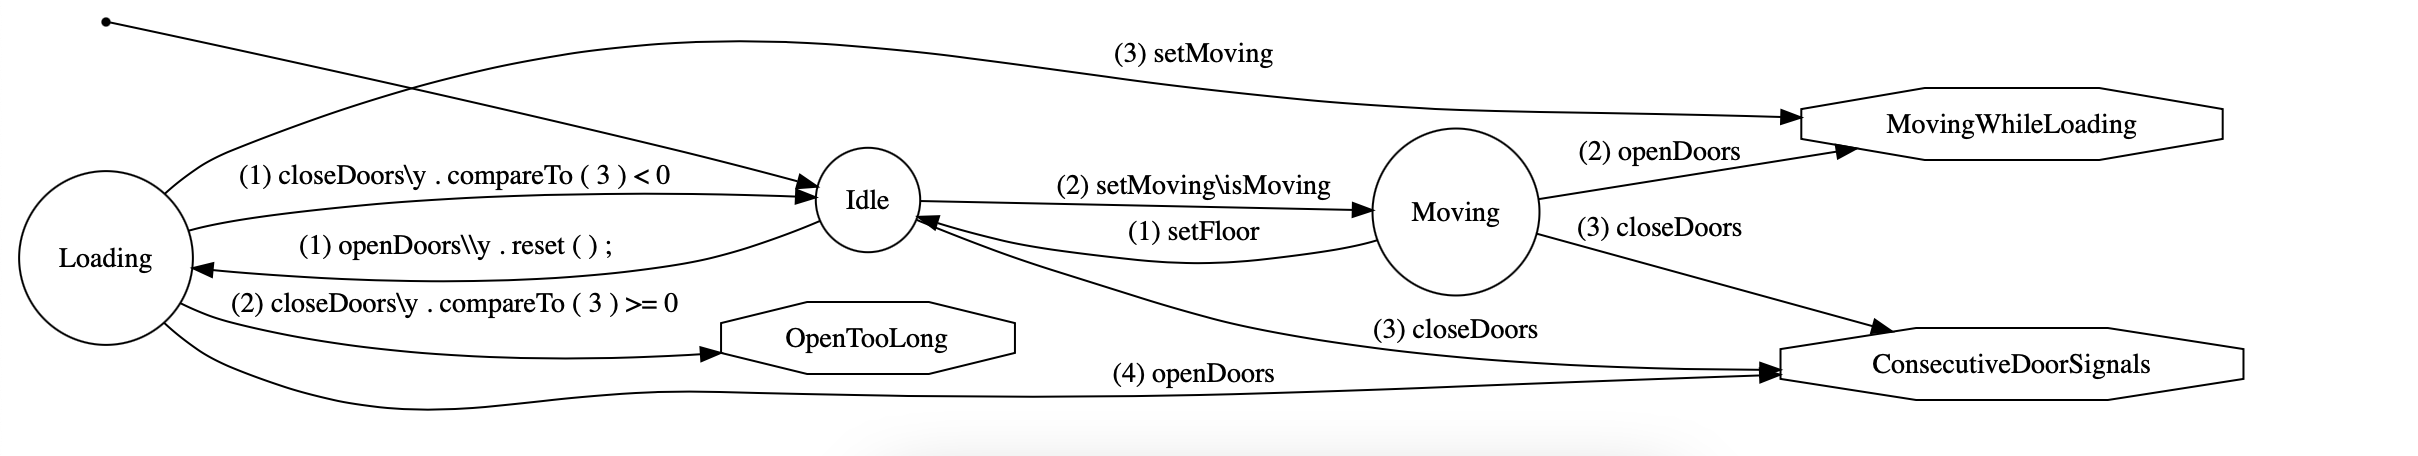
\includegraphics[width=\textwidth,height=\textheight,keepaspectratio]{images/generated-automaton-LiftOpenTimeProperty} % requires the graphicx package
   \caption{Generated automaton for LiftOpenTimeProperty}
   \label{fig:generated-automaton-LiftOpenTimeProperty}
\end{figure}

% Requires the booktabs if the memoir class is not being used
\begin{table}
   \centering
   %\topcaption{Table captions are better up top} % requires the topcapt package
   \begin{tabular}{@{}  |c|c| @{}} % Column formatting, @{} suppresses leading/trailing spac
      \toprule
      Method    & Event \\
      \midrule
      Lift.setMoving(boolean isMoving)   &  goUp/goDown *\\
      Lift.closeDoors()       & closeDoor  \\
      Lift.openDoors()       & openDoor  \\
      Lift.setFloor() & stop    \\
      \bottomrule
   \end{tabular}
   \caption{LiftOpenTimeProperty events table}
   \tablefootnote{*isMoving parameter must be true}
   \label{tab:lift-open-time-property}
\end{table}

To add support for multiple lift, the \texttt{FOREACH} Larva keyword was used to iterate over lift objects. All the event methods resided in the class \textit{Lift.java}. This meant that adding multiple lift support was done by binding the Lift object in the event declarations and then assigning it to the \texttt{FOREACH} object using the \texttt{WHERE} keyword.


\begin{lstlisting}[
language=bash, 
caption={Multiple lift support for LiftOpenProperty}
\label{lst:labelname}
]
setMoving(isMoving) = {Lift l.setMoving(boolean isMoving)} WHERE {lift = l;} 
closeDoors() = {Lift l.closeDoors()} WHERE {lift = l;}
openDoors() = {Lift l.openDoors()} WHERE {lift = l;}
setFloor() = {Lift l.setFloor(*)} WHERE {lift = l;}
\end{lstlisting}

The second property (visual representation in figure \ref{fig:generated-automaton-StartMovingTimeProperty}) is called \texttt{StartMovingTimeProperty} and verifies that the lift start moving in less than 3 seconds after the door closes following a request. A new event was added for the summon request action. The method that corresponds to this event is \texttt{callLiftToFloor}. \\

\begin{figure}
   \centering
   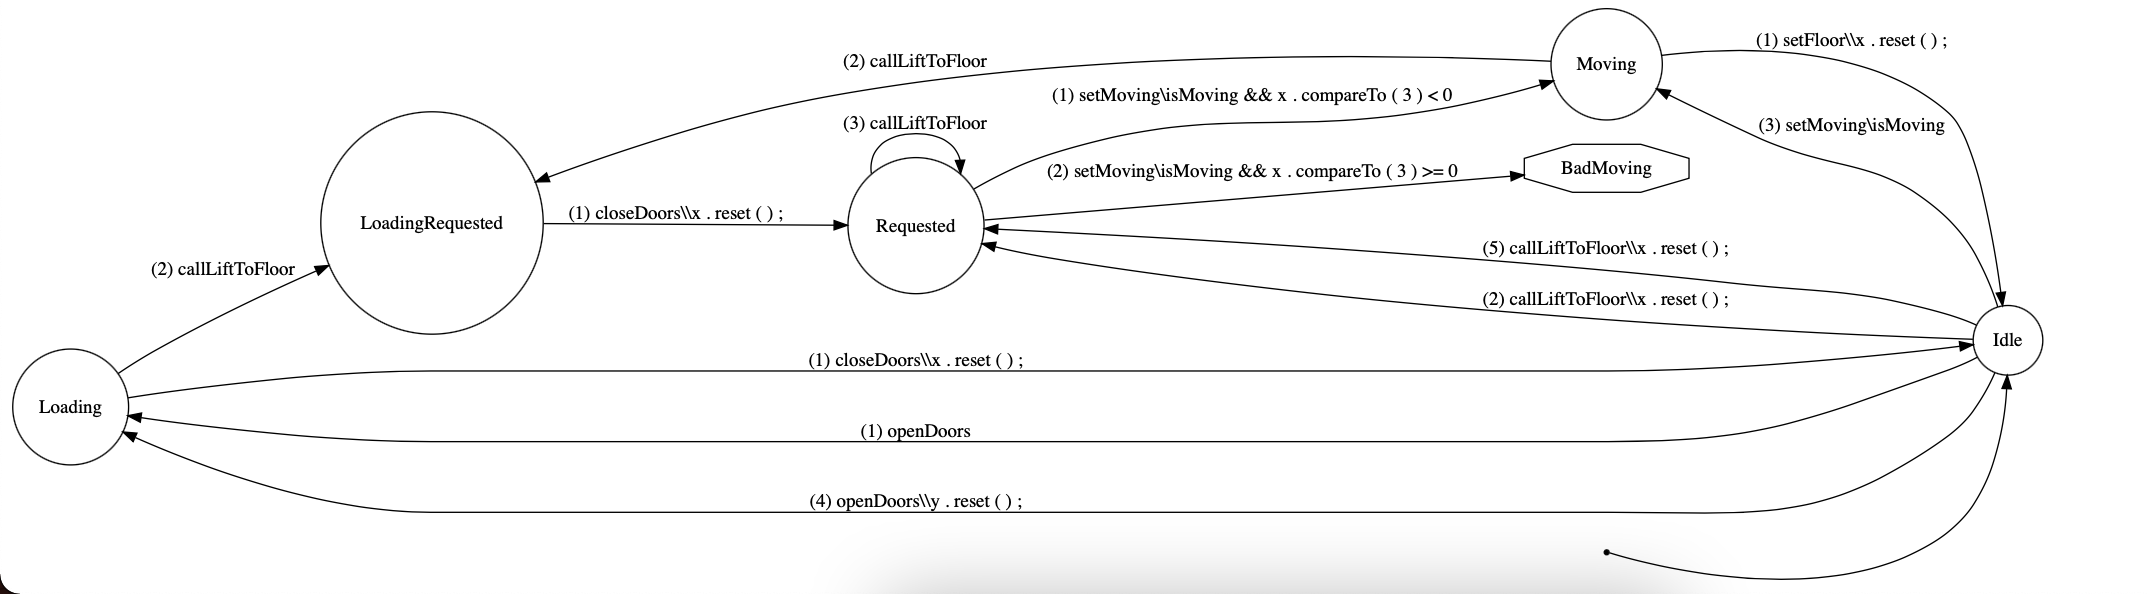
\includegraphics[width=\textwidth,height=\textheight,keepaspectratio]{images/generated-automaton-StartMovingTimeProperty} % requires the graphicx package
   \caption{Generated automaton for StartMovingTimeProperty}
   \label{fig:generated-automaton-StartMovingTimeProperty}
\end{figure}

This method provided some difficulty when switching to adding support for multiple lift verification. The reason being that this method does not reside in the \textit{Lift.java} class. It resided in the \textit{JavaController.java} class. When \texttt{callLiftToFloor} is called, it performs some calculations and then proceeds to execute \texttt{moveLift} with the chosen lift. To find out which lift was called via Larva, the source needed to be edited. The change done was very minimal and does not impact the design of the lift system at all. The \texttt{callLiftToFloor} method signature was changed to return a lift object instead of void. This is then used by Larva by making use of the \texttt{uponReturning} keyword when declaring the event. The whole event declaration is as follows: \newline\texttt{callLiftToFloor(Lift l) = {*callLiftToFloor(*)uponReturning(l)} where {lift = l;}}, where '\texttt{lift}' is the iterated object declared in the FOREACH loop. 

\subsection{Testing}
In the tests shown, one property at a time was tested to make the outputs more legible. Figure \ref{fig:lift-open-test-passed} shows the property \texttt{LiftOpenTimeProperty} running as should. several buttons were pressed and the lift always moved as specified. \\

\begin{figure}
   \centering
   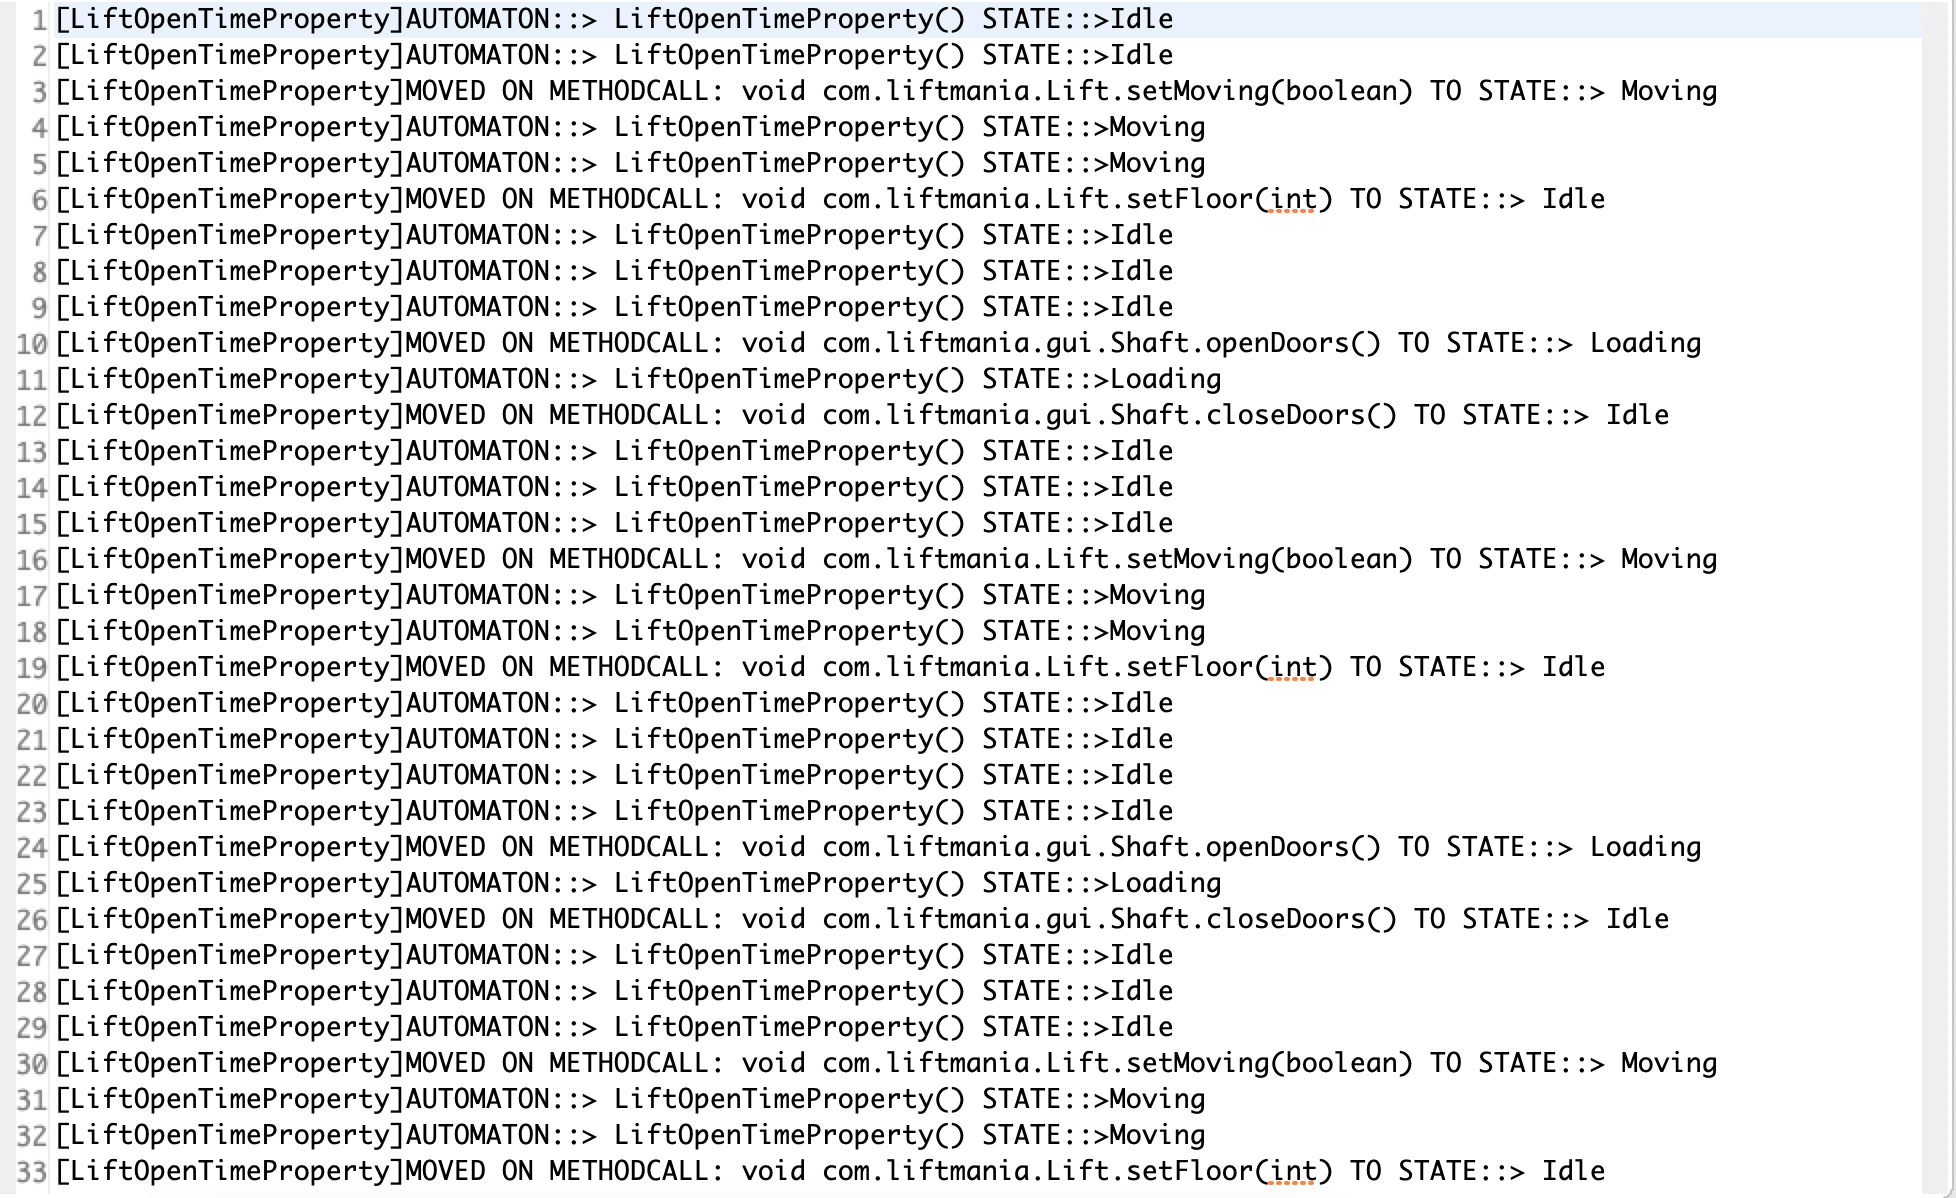
\includegraphics[width=\textwidth,height=\textheight,keepaspectratio]{images/lift-open-test-passed} % requires the graphicx package
   \caption{\texttt{LiftOpenTimeProperty} verified}
   \label{fig:lift-open-test-passed}
\end{figure}

For the second test shown in figure \ref{fig:lift-open-test-failed}, time taken to close the door automatically was changed from the java source code in file \textit{Shaft.java}. The figure shows that verification failed because the door was closing after 3 seconds. \\

\begin{figure}
   \centering
   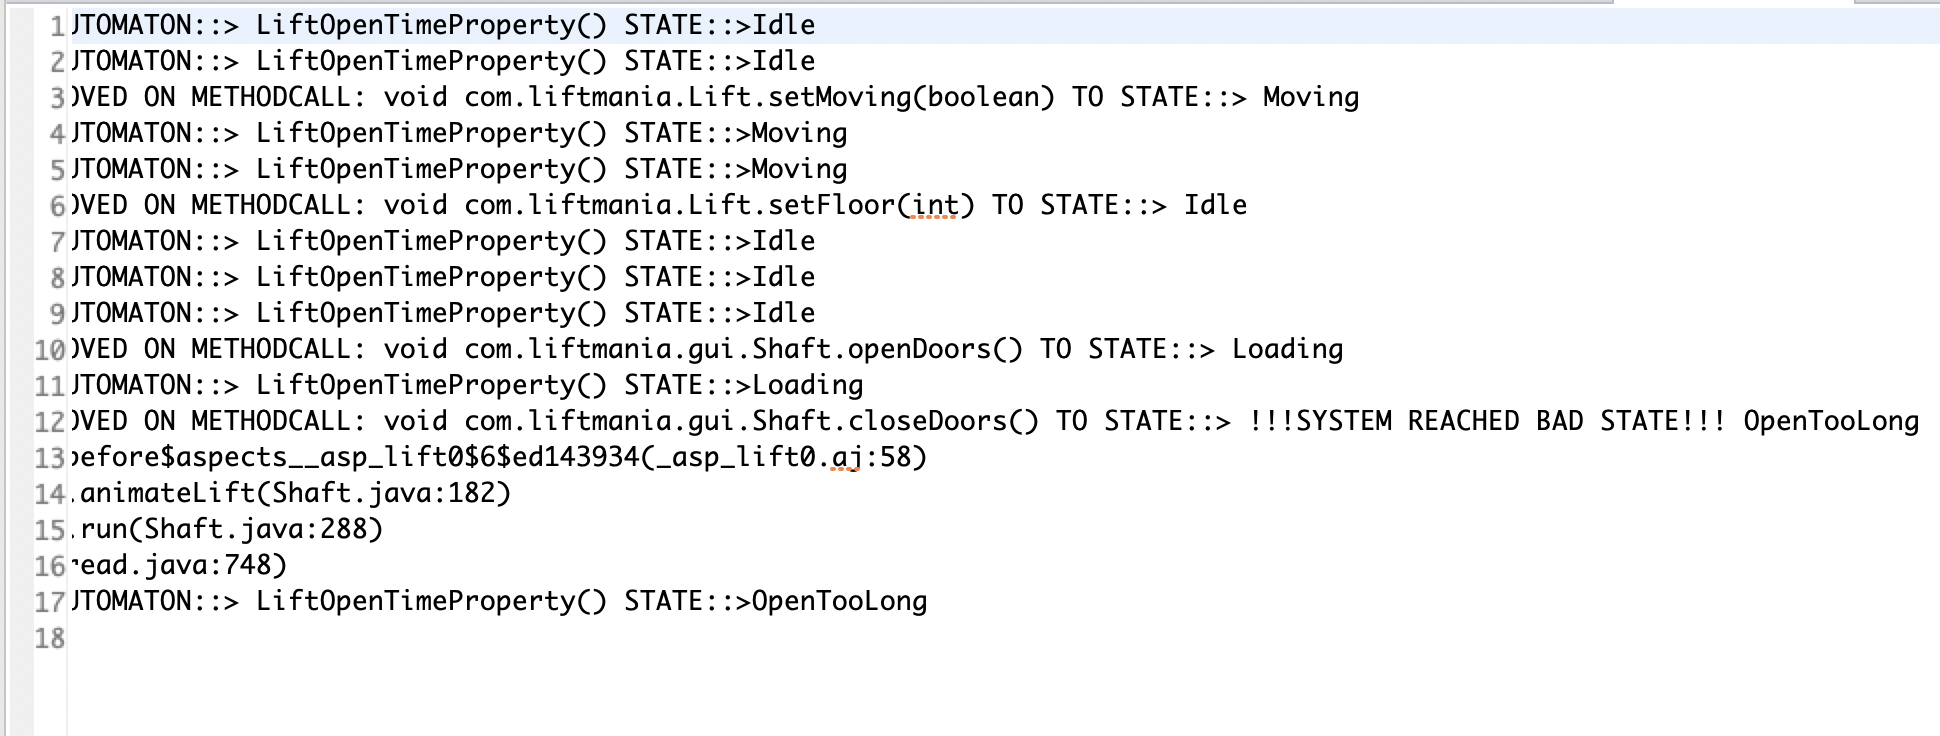
\includegraphics[width=\textwidth,height=\textheight,keepaspectratio]{images/lift-open-test-failed} % requires the graphicx package
   \caption{\texttt{LiftOpenTimeProperty} failed}
   \label{fig:lift-open-test-failed}
\end{figure}

Referirng to figure \ref{fig:lift-open-test-multiple} the third test shown, displays the verification being conducted on several (three) lifts. Identifiers are used to differentiate the multiple lifts being verified. \\

\begin{figure}
   \centering
   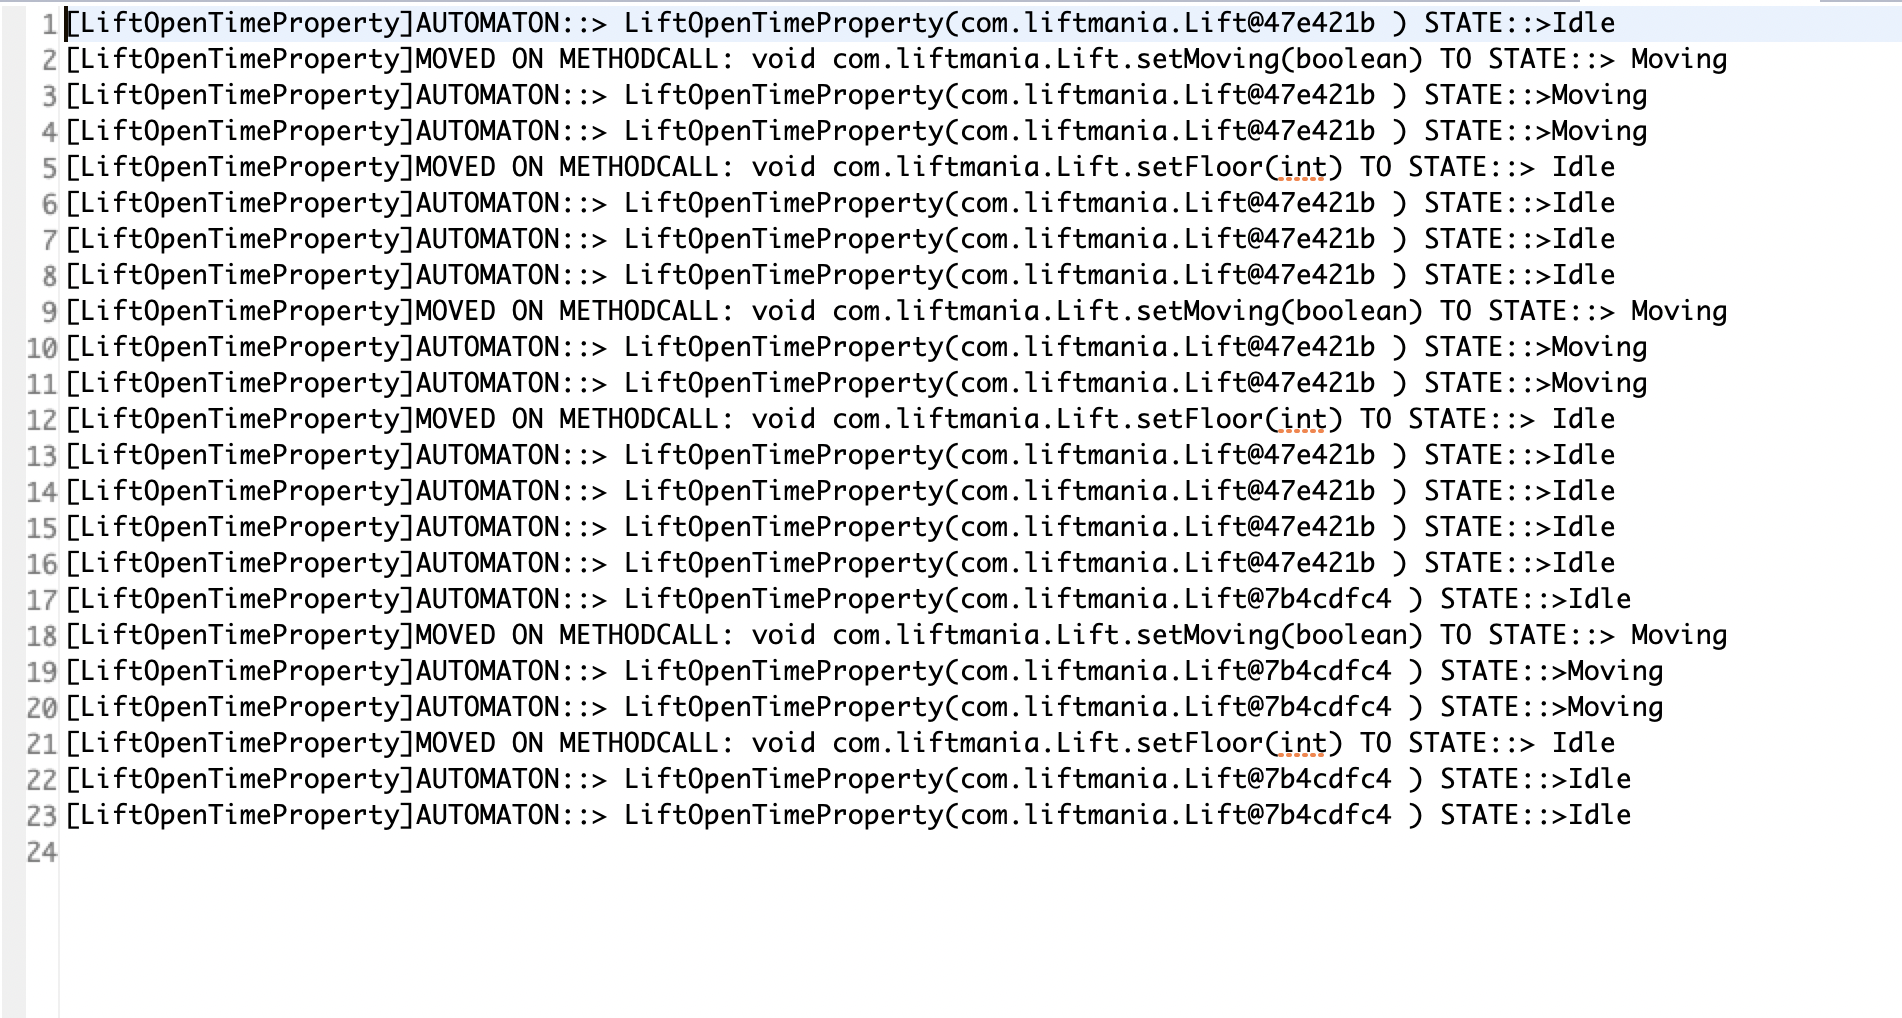
\includegraphics[width=\textwidth,height=\textheight,keepaspectratio]{images/lift-open-test-multiple} % requires the graphicx package
   \caption{\texttt{LiftOpenTimeProperty} on several lifts}
   \label{fig:lift-open-test-multiple}
\end{figure}

Figure \ref{fig:start-moving-time-property-several} shows the fourth documented test. This test shows the verification of the \texttt{StartMovingTimeProperty} working on more than one lift. To make the output more clear, the \texttt{LiftOpenTimeProperty} was removed from the script to focus only on the property discussed. \\
\begin{figure}
   \centering
   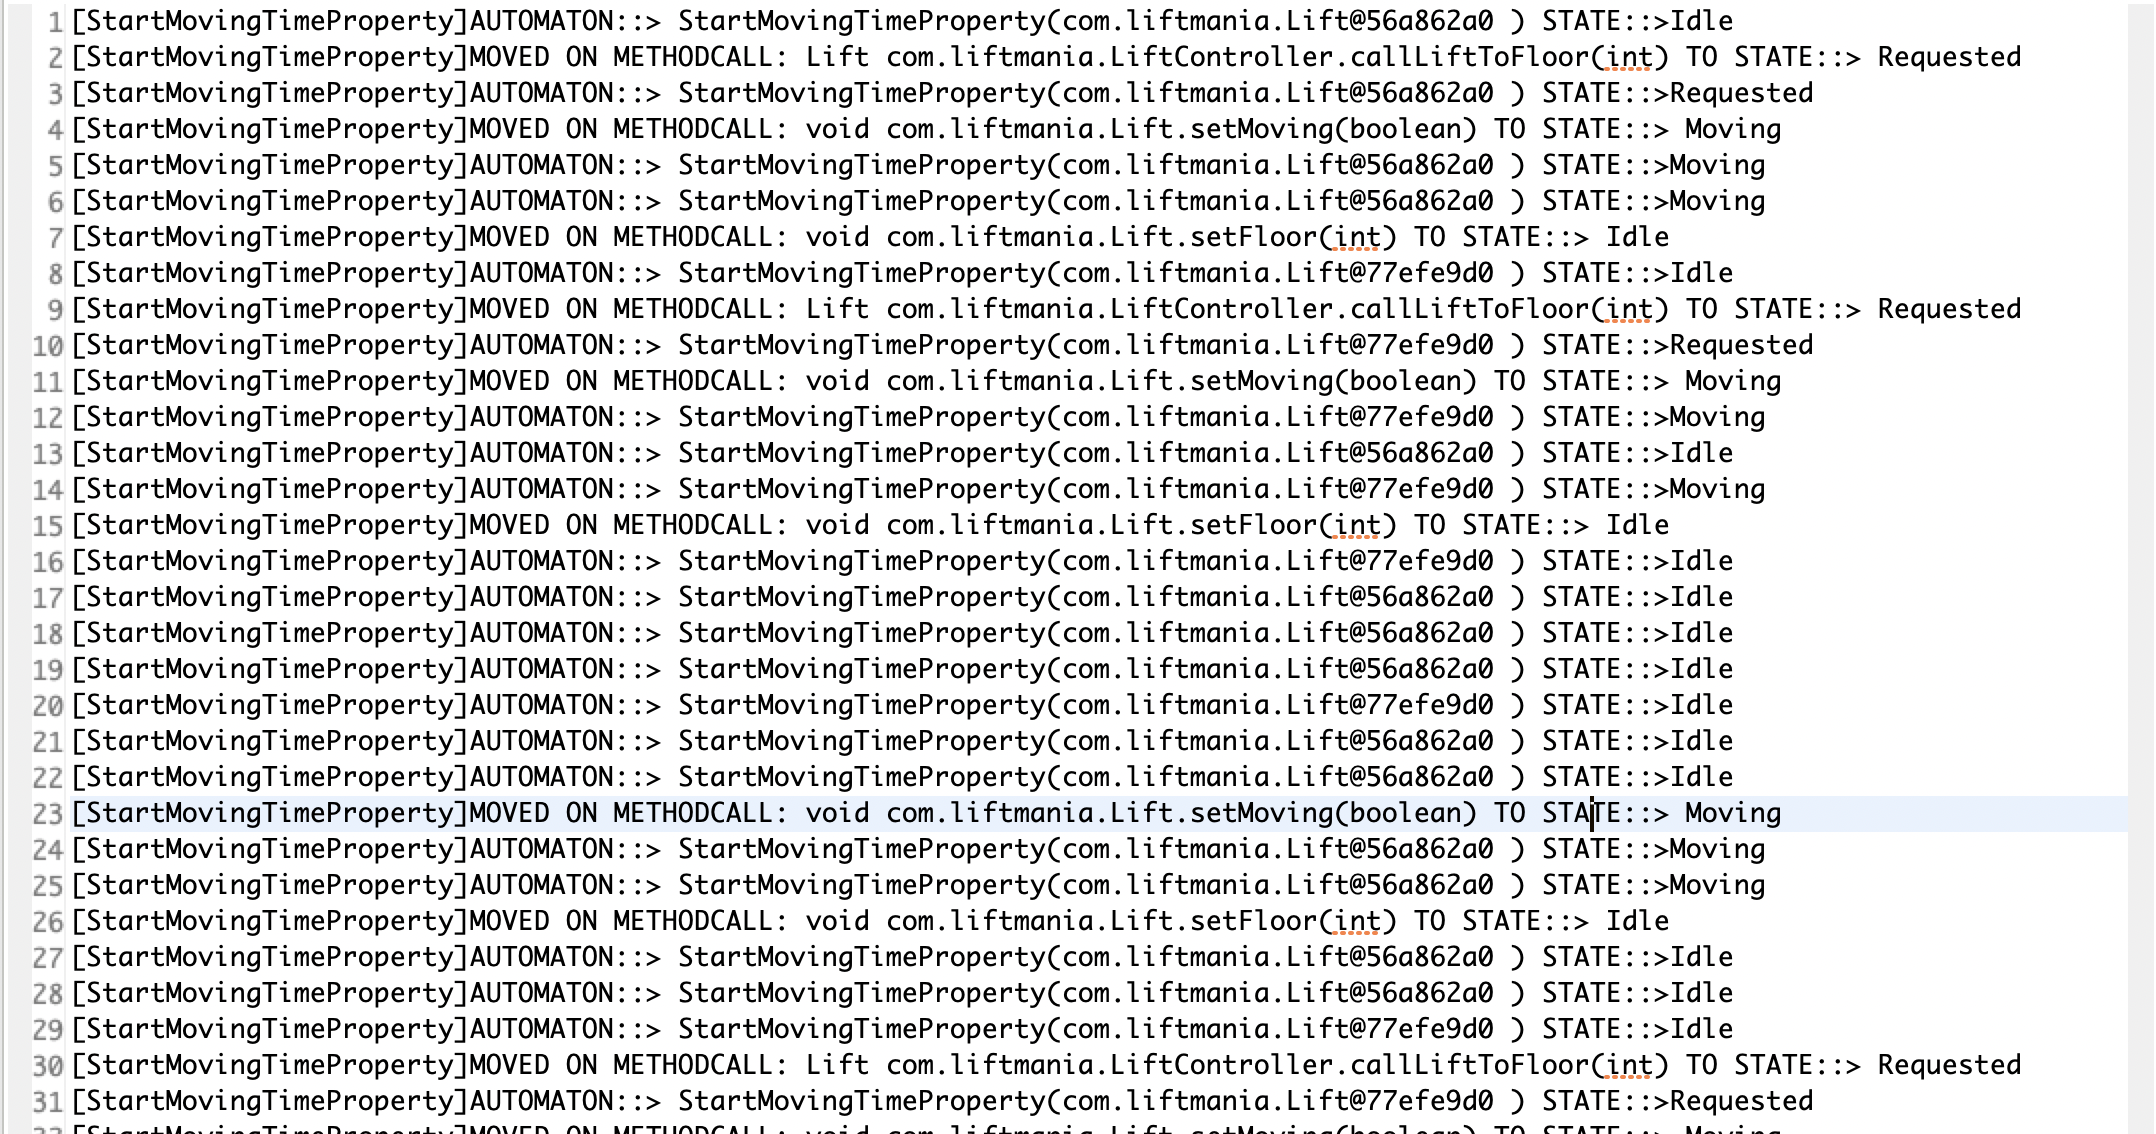
\includegraphics[width=\textwidth,height=\textheight,keepaspectratio]{images/start-moving-time-property-several} % requires the graphicx package
   \caption{\texttt{StartMovingTimeProperty} on several lifts}
   \label{fig:start-moving-time-property-several}
\end{figure}

A failure was also induced for this property. The \texttt{animateLift} method in \textit{Shaft.java} was edited to wait three seconds before starting to move the lift. The added code can be seen in figure \ref{fig:start-moving-time-property-failure-edit}. As expected, this caused the verification to fail. The output can be seen in figure \ref{fig:start-moving-time-property-failed}

\begin{figure}
   \centering
   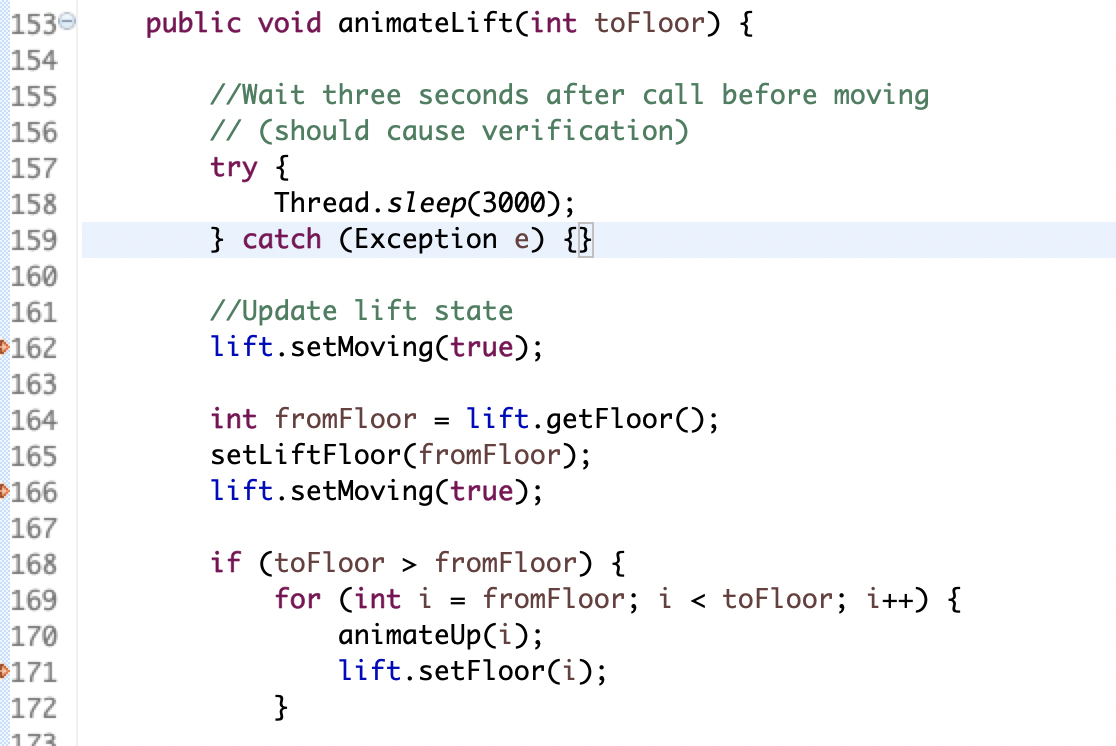
\includegraphics[width=\textwidth,height=\textheight,keepaspectratio]{images/start-moving-time-property-failure-edit} % requires the graphicx package
   \caption{Added code to stop for three seconds before starting to move lift in \textit{Shaft.java}}
   \label{fig:start-moving-time-property-failure-edit}
\end{figure}

\begin{figure}
   \centering
   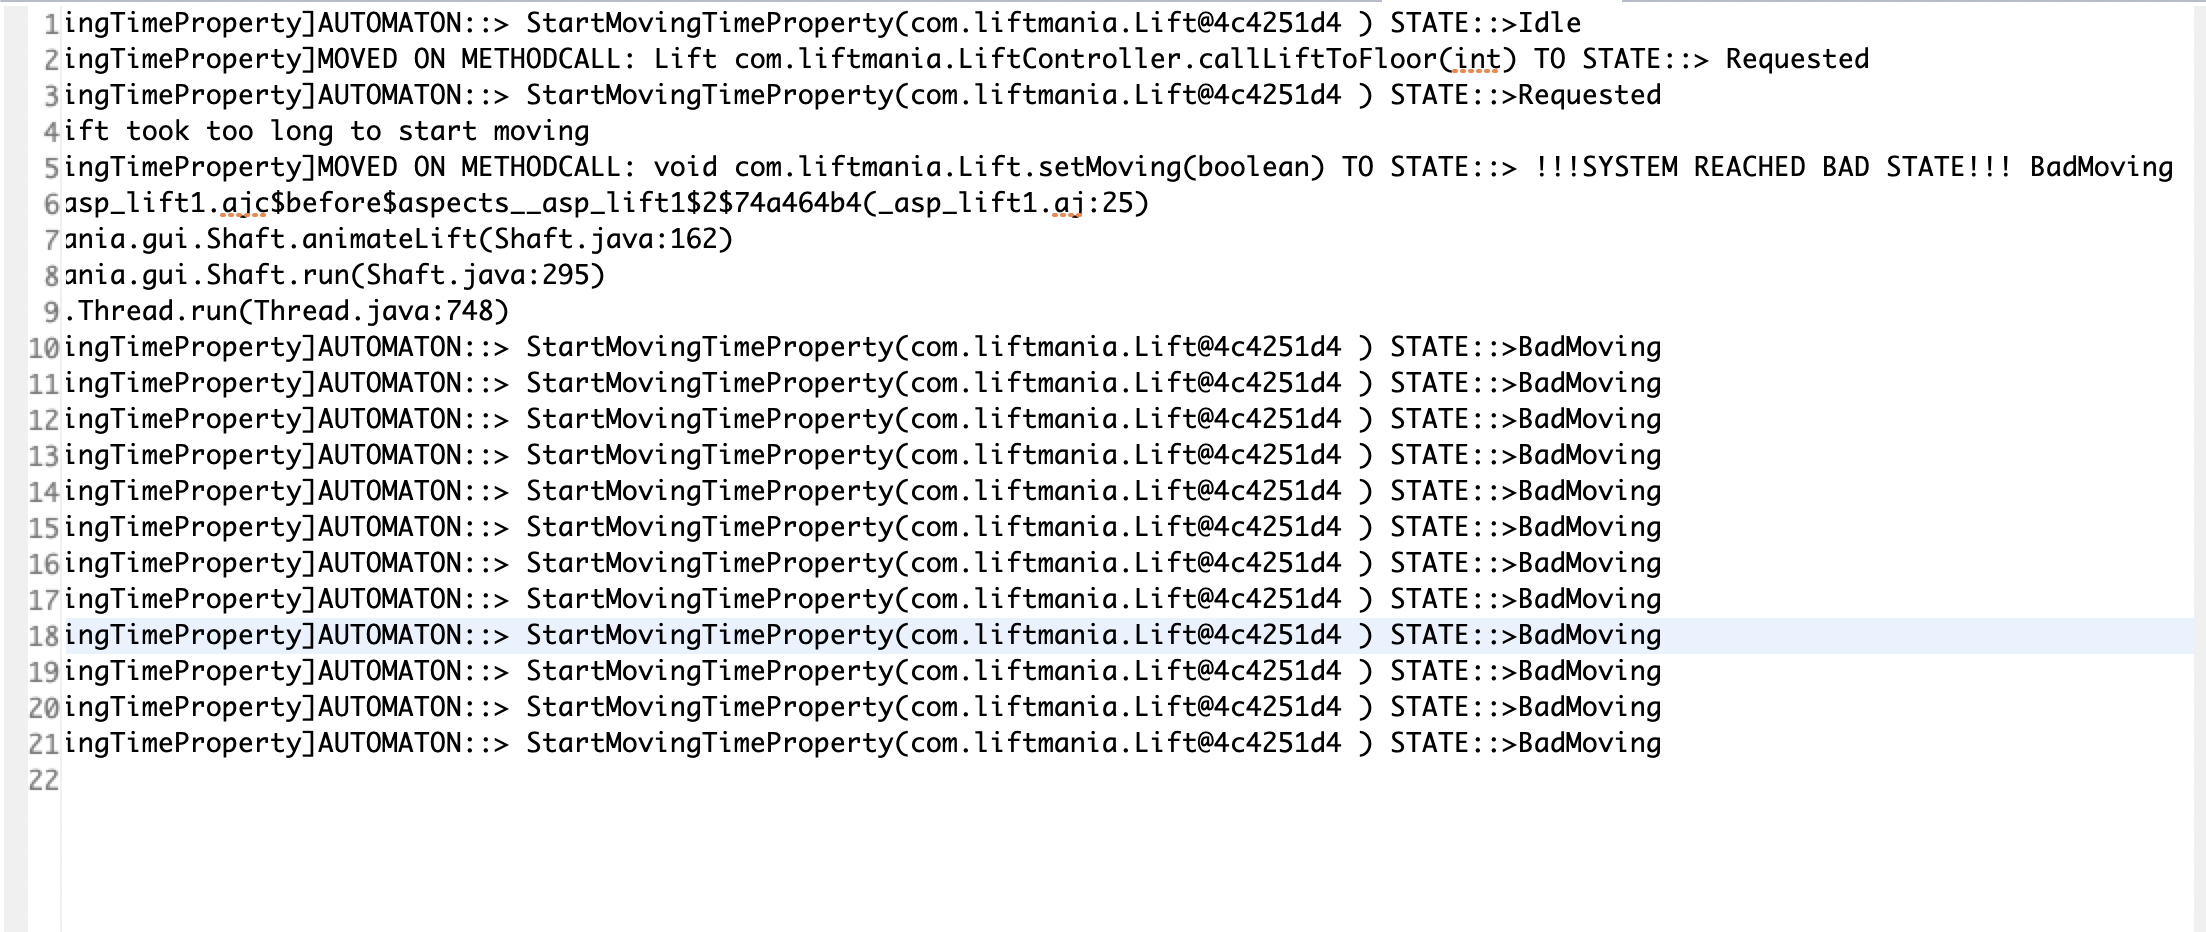
\includegraphics[width=\textwidth,height=\textheight,keepaspectratio]{images/start-moving-time-property-failed} % requires the graphicx package
   \caption{\texttt{StartMovingTimeProperty} failure}
   \label{fig:start-moving-time-property-failed}
\end{figure}

The final test showcased in this section can be seen in figure \ref{fig:all-properties}. This shows all the properties being run at once for several lifts. 

\begin{figure}
   \centering
   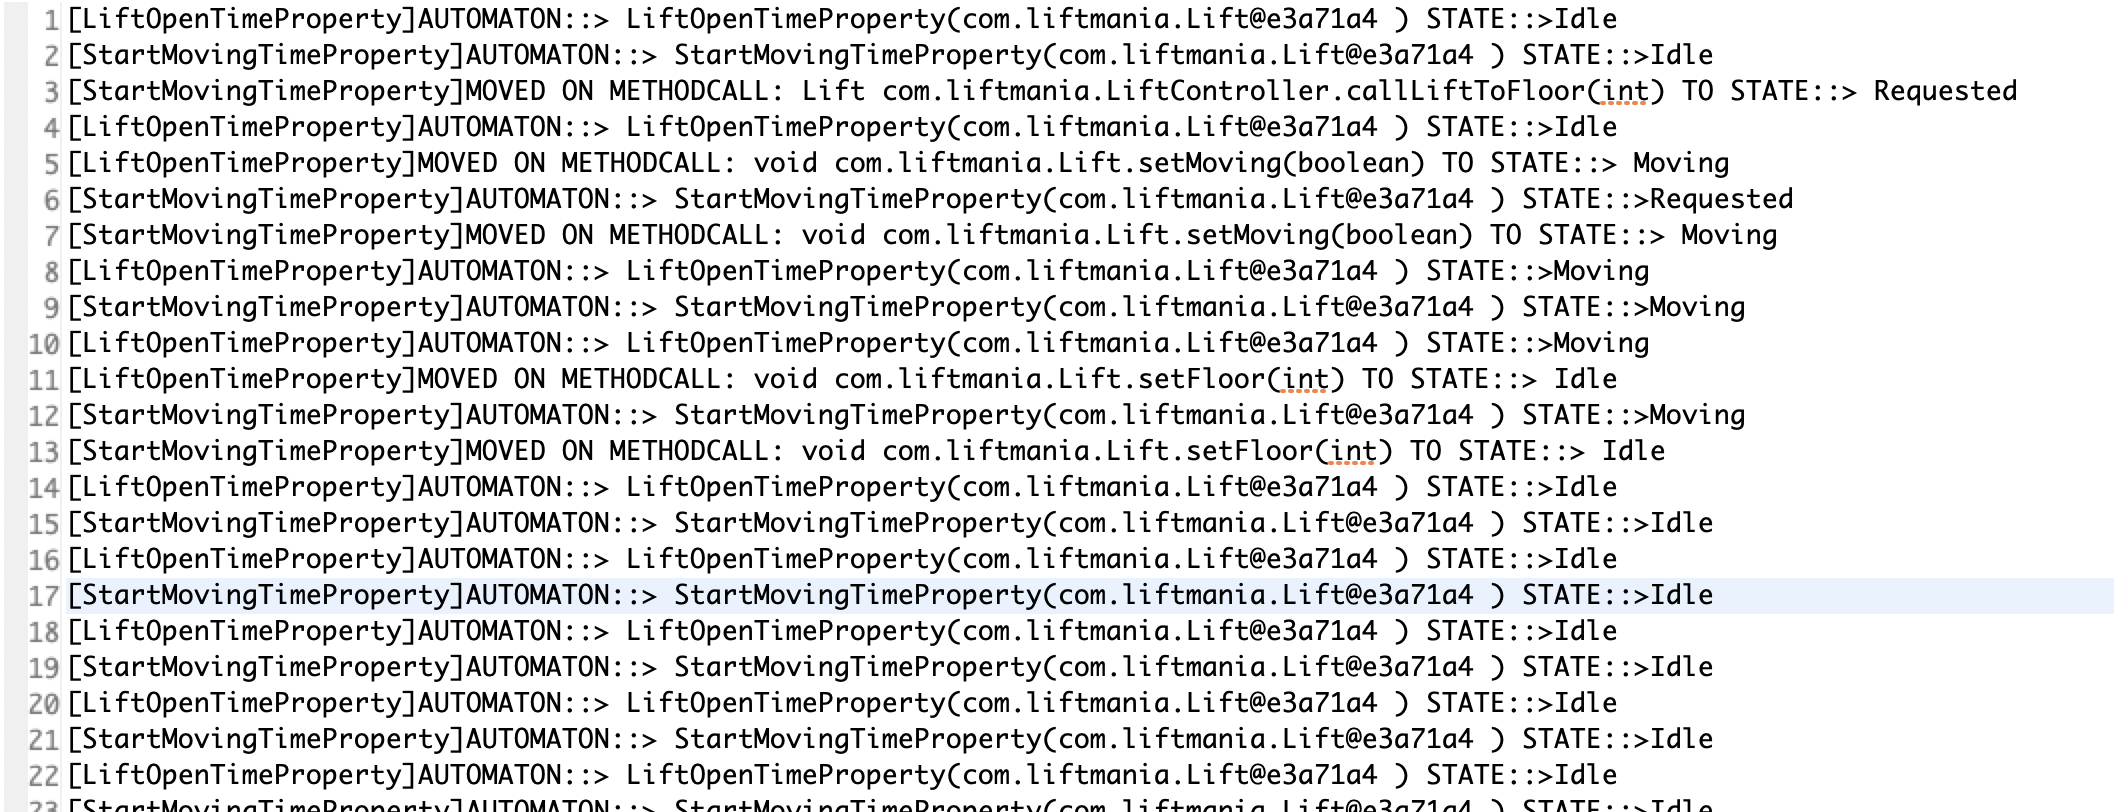
\includegraphics[width=\textwidth,height=\textheight,keepaspectratio]{images/all-properties} % requires the graphicx package
   \caption{All properties}
   \label{fig:all-properties}
\end{figure}

\subsection{Larva script improvements}
The script developed is not perfect. One flaw with the system is that requests are only summon requests. This means that only buttons on floors are verified. The reason for this decision lies in the java source code for the Lift system. As can be seen in figure \ref{fig:floor-request-code} was a button is pressed, it is registered as a \texttt{move} action. As opposed to using a function similar to summon requests where \texttt{callLiftToFloor} is used. \\

One possible way to circumvent this problem would have been to iterate over \texttt{Shaft} objects rather than \texttt{Lift} object as the script does currently. This would have most likely work since each shaft corresponds to a single that resides in it. The \textit{Shaft.java} class also contains \texttt{openDoors()} and \texttt{closeDoors()} methods similar to the \textit{Lift.java} class. Movement events would have been recognised by the \texttt{animateUp()} and \texttt{animateDown()} present in \textit{Shaft.java}. Finally, stopping would have been recognised by the \texttt{animationPause()} method. Iteration over the \texttt{Shaft} objects would enable the script to track which shaft floor buttons were pressed. 

\begin{figure}
   \centering
   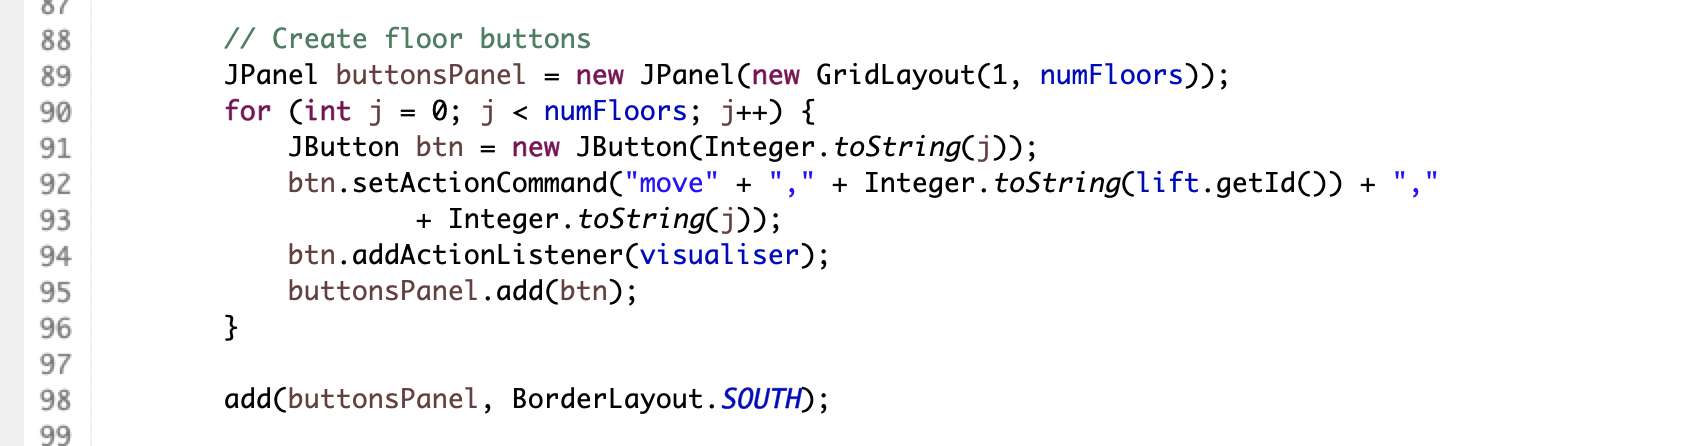
\includegraphics[width=\textwidth,height=\textheight,keepaspectratio]{images/floor-request-code} % requires the graphicx package
   \caption{Floor request button code}
   \label{fig:floor-request-code}
\end{figure}



\section{Model-Based Testing}
For model based testing ModelJUnit was used. Importing the project with maven provided several difficulties and wasted efforts. As a result, the ModelJUnit jar file was used. Also, the Intellij IDE was used for this task instead of eclipse. \\


\subsection{BasicLiftModel}
The previous automata were used for Model-based testing. Using this model, internal variables and states are updated and compared to the system under test (SUT). This workflow can be seen visually in figure \ref{fig:model-based-testing-diag}. This model  also checks for temporal some temporal properties for example trying to open a lift that is already open. This is done via  assertions at the start of the method to check the current state. \\

\begin{figure}
   \centering
   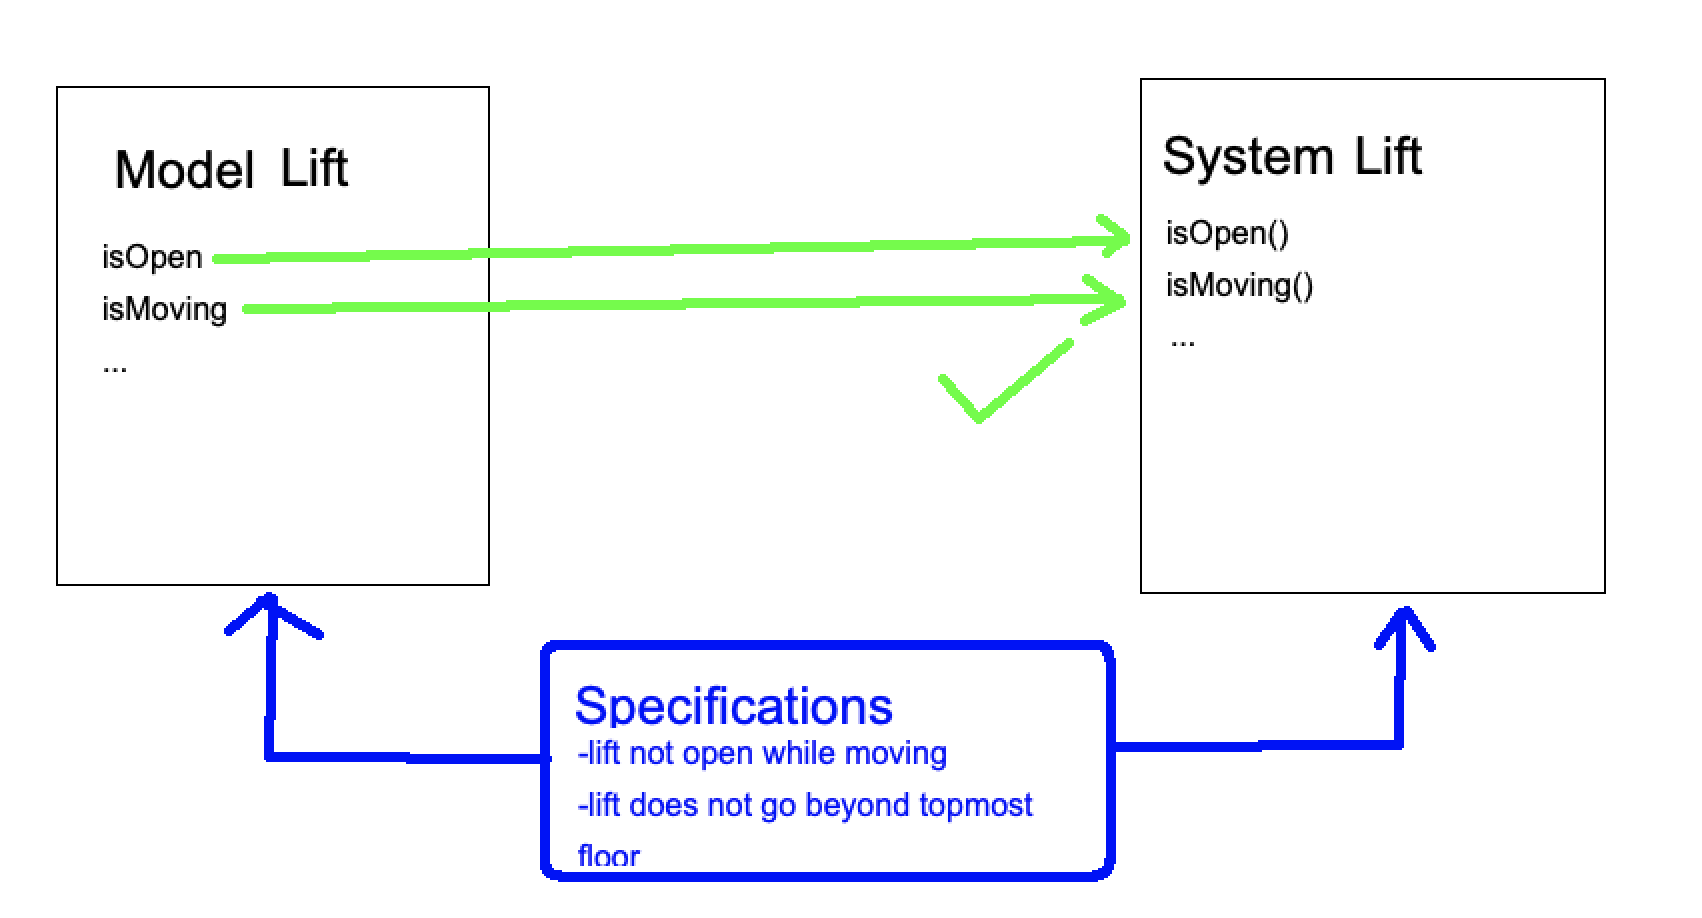
\includegraphics[width=\textwidth,height=\textheight,keepaspectratio]{images/model-based-testing-diag} % requires the graphicx package
   \caption{Model based testing diagram}
   \label{fig:model-based-testing-diag}
\end{figure}

The first model implemented is based on the automaton seen in \ref{fig:FSA}. The variables that the model keeps track of are shown in figure \ref{fig:BasicLiftModel-variables}. When the flow enters a state in the model, these variables are updated and matched with the SUT's variables via the assert method. Two types of assert methods are used in this model: \newline
\texttt{Assert.assertEquals("Model does not match SUT: Moving", isMoving, lift.isMoving());} \newline
\texttt{Assert.assertFalse("Moved with door open", lift.isOpen());}
The first one is comparing a variable of the model with a variable of the SUT while the second is comparing a verifying that a variable of SUT is in accordance with the current state.\\ 

\begin{figure}
   \centering
   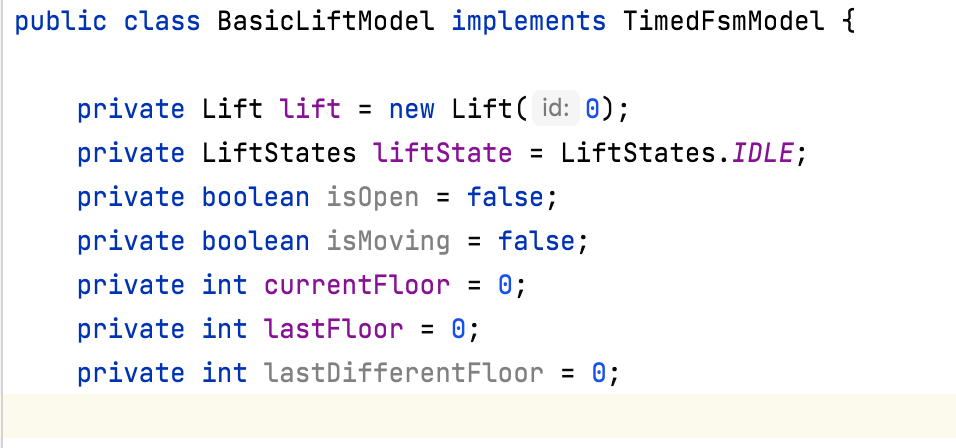
\includegraphics[width=\textwidth,height=\textheight,keepaspectratio]{images/BasicLiftModel-variables} % requires the graphicx package
   \caption{BasicLiftModel variables}
   \label{fig:BasicLiftModel-variables}
\end{figure}

The tests provided full coverage for this model. This can be seen in figure \ref{fig:BaseLiftModel-coverage}. The Lift system passes the test. The \textit{Lift.java} was then edited with faulty code. The code added was a \texttt{openDoors()} call in the \texttt{moveLift()} method. This caused the test to fail as can be seen in figure \ref{fig:BasicLiftModel-fail}. \\

\begin{figure}
   \centering
   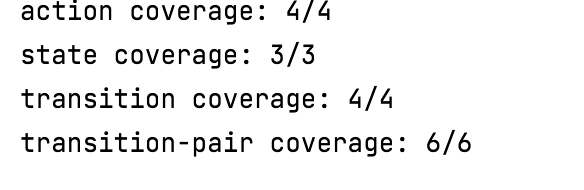
\includegraphics[width=\textwidth,height=\textheight,keepaspectratio]{images/BaseLiftModel-coverage} % requires the graphicx package
   \caption{BaseLiftModel test coverage}
   \label{fig:BaseLiftModel-coverage}
\end{figure}

\begin{figure}
\centering
\begin{subfigure}{.5\textwidth}
  \centering
  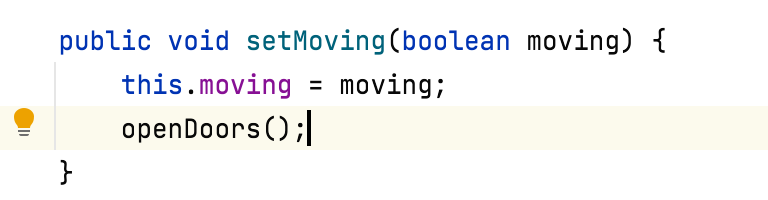
\includegraphics[width=\linewidth]{images/BasicLiftModel-fail-code}
  \caption{Code edit}
\end{subfigure}%
\begin{subfigure}{.5\textwidth}
  \centering
  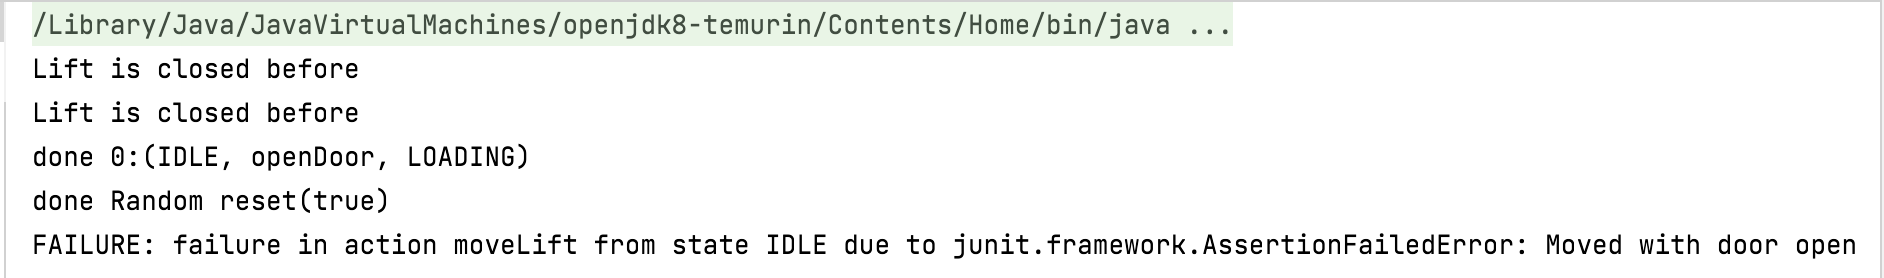
\includegraphics[width=\linewidth]{images/BasicLiftModel-fail-output}
  \caption{Output}
\end{subfigure}
\caption{BasicLiftModel test failure}
\label{fig:BasicLiftModel-fail}
\end{figure}

\subsection{LiftTimeModel}
To test time properties another model was created. The provided lift system did not include a clock class so time could not be mocked easily by ModelJUnit. As a result, inline java code had to be used, for example \texttt{Thread.sleep}. \\

This part was not fully implemented. Due to problems found with driving the \texttt{LiftController} class. The aim was to make the SUT run \texttt{LiftController.moveLift(...)} and simulate it from the model side to match the correct times for example verifying that the door stays open for less than 3 seconds. However a problem arose where the method \texttt{LiftController.moveLift(...)} was not taking the necessary time to run. It should have taken the function at least 2000 milliseconds since it contains a \texttt{thread.sleep} however upon debugging it was shown to take only 2 milliseconds maximum. The code to time the function can be seen in the \texttt{moveLift()} action in \textit{LiftTimeModel} class or in listing \ref{lst:time-liftcontroller}.

\begin{lstlisting}[
caption={FSA definition}
\label{lst:time-liftcontroller}
tabsize = 4, %% set tab space width
showstringspaces = false, %% prevent space marking in strings, string is defined as the text that is generally printed directly to the console
numbers = left, %% display line numbers on the left
commentstyle = \color{green}, %% set comment color
keywordstyle = \color{blue}, %% set keyword color
stringstyle = \color{red}, %% set string color
rulecolor = \color{black}, %% set frame color to avoid being affected by text color
basicstyle = \small \ttfamily , %% set listing font and size
breaklines = true, %% enable line breaking
numberstyle = \tiny,
language=java
]
 liftState = LiftStates.MOVING;
        startMoving = System.currentTimeMillis();


        if (currentFloor == 0 ) {
            liftController.moveLift(0, 5);
        } else {
            liftController.moveLift(0, 0);
        }

        System.out.print("Time taken: ");
        System.out.println(System.currentTimeMillis() - startMoving);

\end{lstlisting}



\section{Runtime Verification and Testing}
For this task, executing RV and model-based testing at the same time was required. This means that this task is combining the artefacts of task 2 and task 3 together.  The eclipse IDE needed to be used again so that the LARVA plugin could be used. The two tasks (2 and 3) contain a different structure. This is because the provided project structure by the respective IDE was used. This resulted in task 4 containing a combination of the structure of the two tasks. Table \ref{tab:packages-structure} shows the package structure of each task to make things clearer. Similarly, the directory trees can be seen in figure \ref{fig:directories-trees}. \\

\begin{table}
   \centering
   %\topcaption{Table captions are better up top} % requires the topcapt package
   \begin{tabular}{@{}  |c|c| @{}} % Column formatting, @{} suppresses leading/trailing spac
      \toprule
      Task   & Packages \\
      \midrule
      Task 2  &  com.liftmania\\
      Task 3 & main.java.com.liftmania  \\
      & test.java.com.liftmania\\
      Task 4  & main.java.com.liftmania\\
      & test.java.com.liftmania\\
      \bottomrule
   \end{tabular}
   \caption{LiftOpenTimeProperty events table}
   \label{tab:packages-structure}
\end{table}

\begin{figure}
\centering
\begin{subfigure}{.5\textwidth}
  \centering
  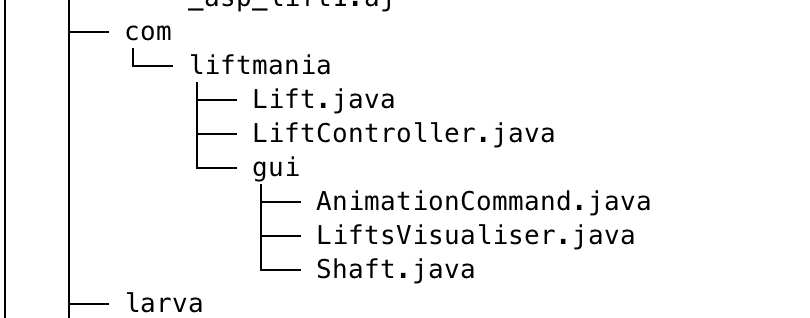
\includegraphics[width=\linewidth]{images/task2-tree}
  \caption{Task 2}
\end{subfigure}%
\begin{subfigure}{.5\textwidth}
  \centering
  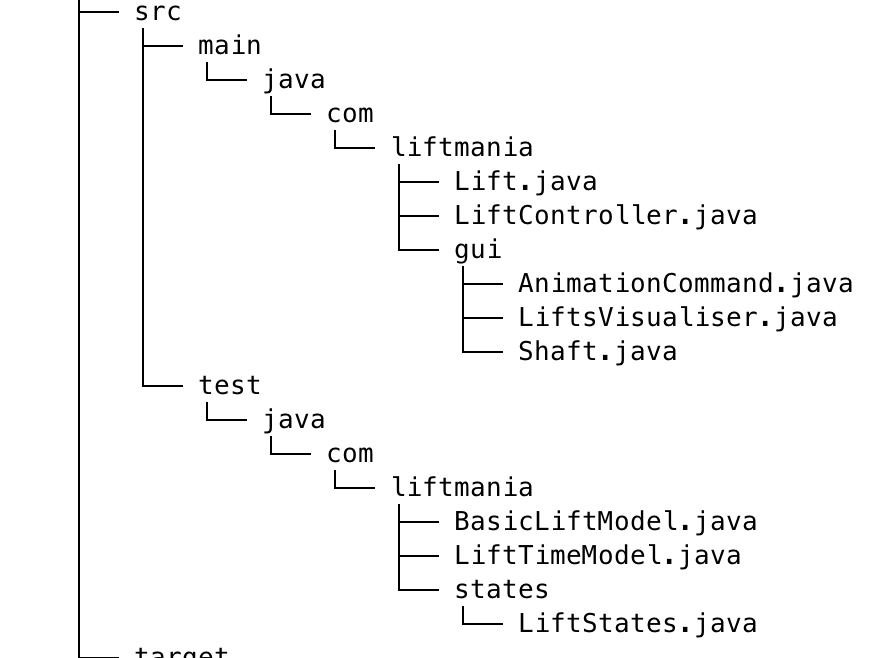
\includegraphics[width=\linewidth]{images/task3-tree}
  \caption{Task 3}
\end{subfigure}
\begin{subfigure}{.5\textwidth}
  \centering
  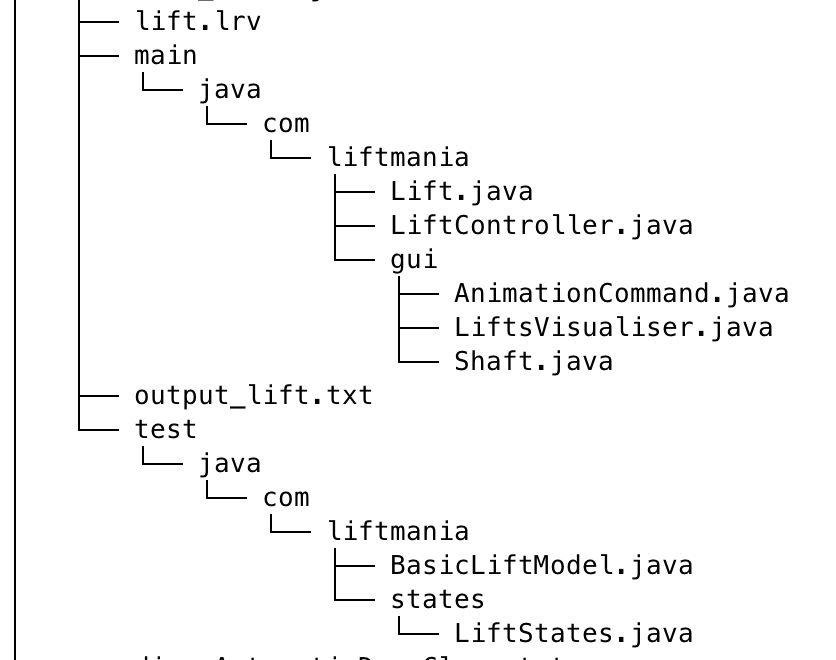
\includegraphics[width=\linewidth]{images/task4-tree}
  \caption{Task 4}
\end{subfigure}
\caption{Directory trees for each task}
\label{fig:directories-trees}
\end{figure}

One difference between RV and testing is that in runtime verification, the user/tester controls the system as usual while RV is done in the background independent of what actions the user does. Meanwhile, in testing, the system is driven by the tests i.e., the tests decide what flow the system follows. In this task, RV is used but it is executed on the system driven by the tests. For example the tests run the method \texttt{moveLift()} and the RV 'catches' this and change the state accordingly. Since the Larva script and Model JUnit tests are based on the same automata, the same states should be visited. This can be seen figuratively in figure \ref{fig:tasks-diagrams} \\

\begin{figure}
\centering
\begin{subfigure}{.5\textwidth}
  \centering
  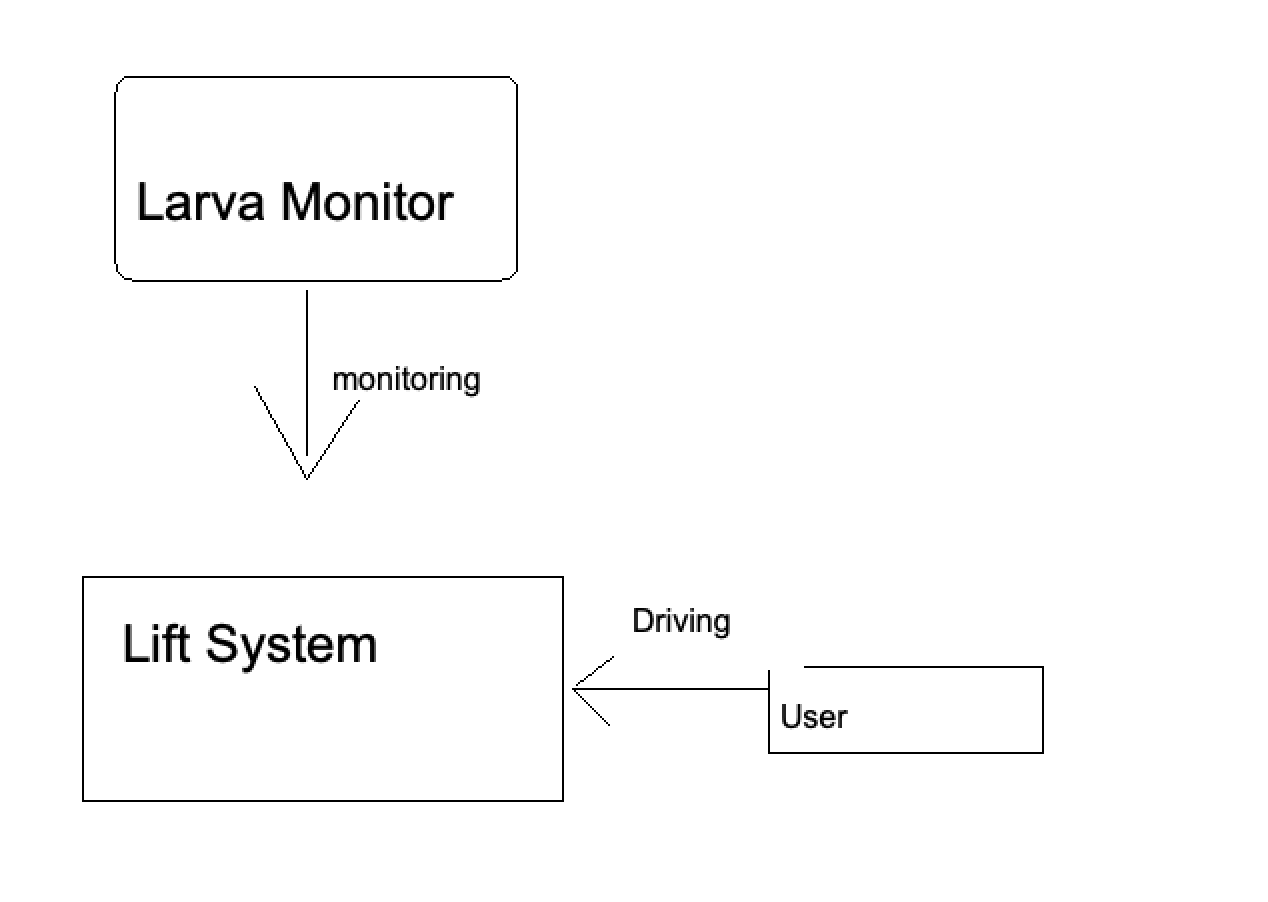
\includegraphics[width=\linewidth]{images/task2-diagram}
  \caption{Task 2}
\end{subfigure}%
\begin{subfigure}{.5\textwidth}
  \centering
  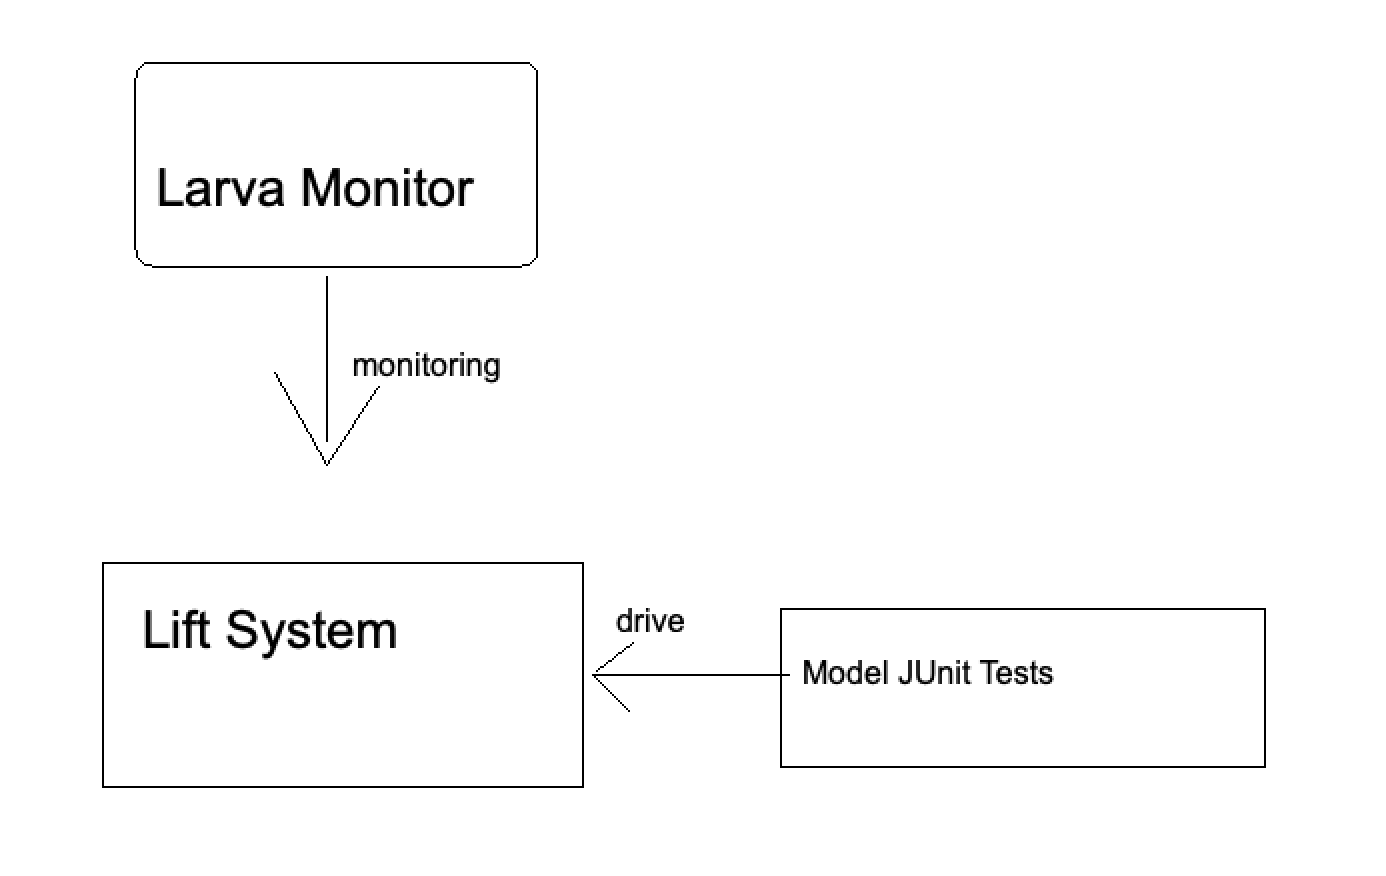
\includegraphics[width=\linewidth]{images/task4-diagram}
  \caption{Task 4}
\end{subfigure}
\caption{Larva diagram for each task}
\label{fig:tasks-diagrams}
\end{figure}

To test this setup, some faults where introduced to investigate wether larva ends in a bad state. In the first test shown in this section, the \texttt{StartMovingTimeProperty} was removed to make analysis of the Larva output less simpler. Then, the Model JUnit method that calls the \texttt{closeDoors()} was modified to wait 4 seconds before proceeding to close the doors. As expected, this resulted in a bad state being reached. The modified code and the result can be seen in figure \ref{fig:larva-test-fail}. \\

The second test discussed in this section can be seen in figure \ref{fig:larva-test-fail-2}. In this test the ModelJunit code was edited to open the doors before moving. Assertions that checked for this bug were commented out so that the program does not stop running. The Larva script successfully detected the errors. \\

\begin{figure}
\centering
\begin{subfigure}{.5\textwidth}
  \centering
  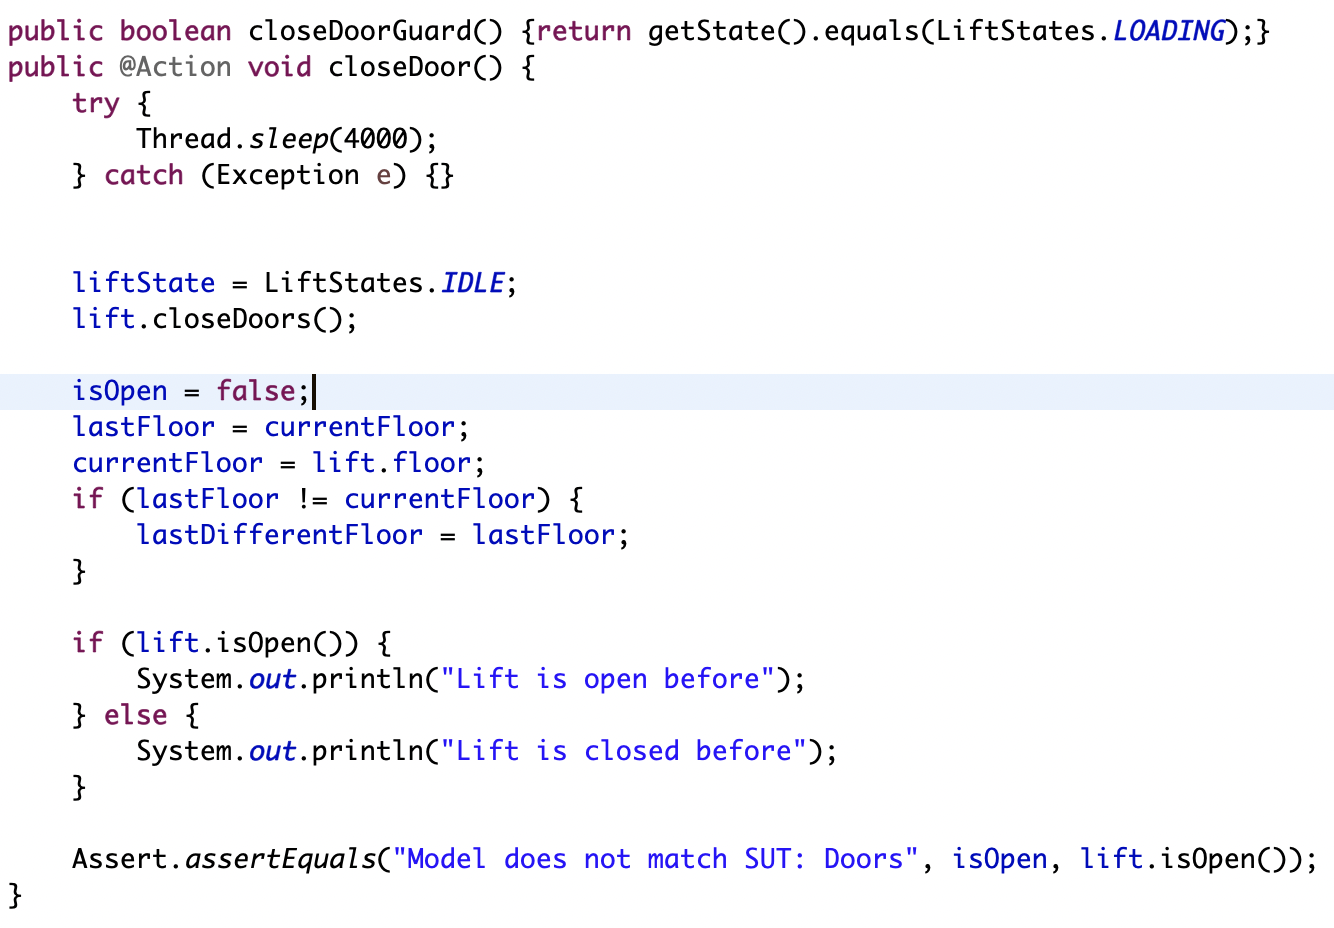
\includegraphics[width=\linewidth]{images/larva-test-fail-code}
  \caption{Modified code in ModelJUnit}
\end{subfigure}%
\begin{subfigure}{.5\textwidth}
  \centering
  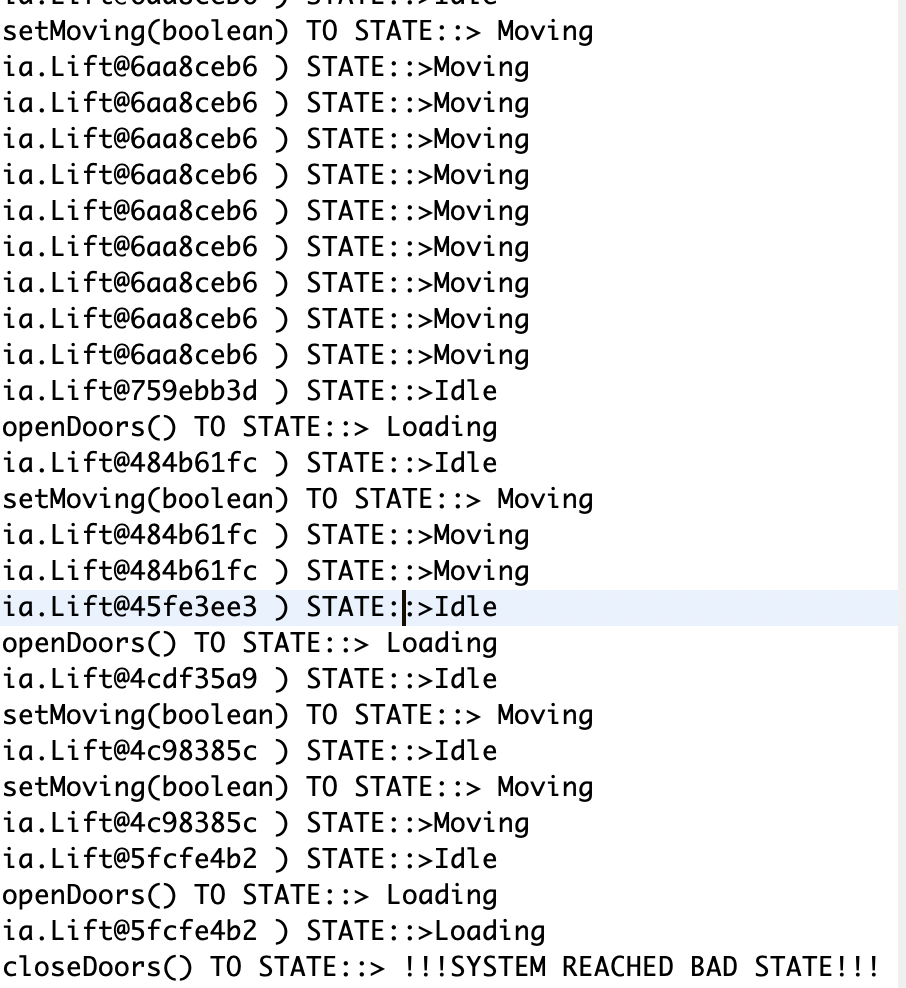
\includegraphics[width=\linewidth]{images/larva-test-fail-output}
  \caption{Larva output}
\end{subfigure}
\caption{RV reaches bad state from test example 1}
\label{fig:larva-test-fail}
\end{figure}

\begin{figure}
\centering
\begin{subfigure}{.5\textwidth}
  \centering
  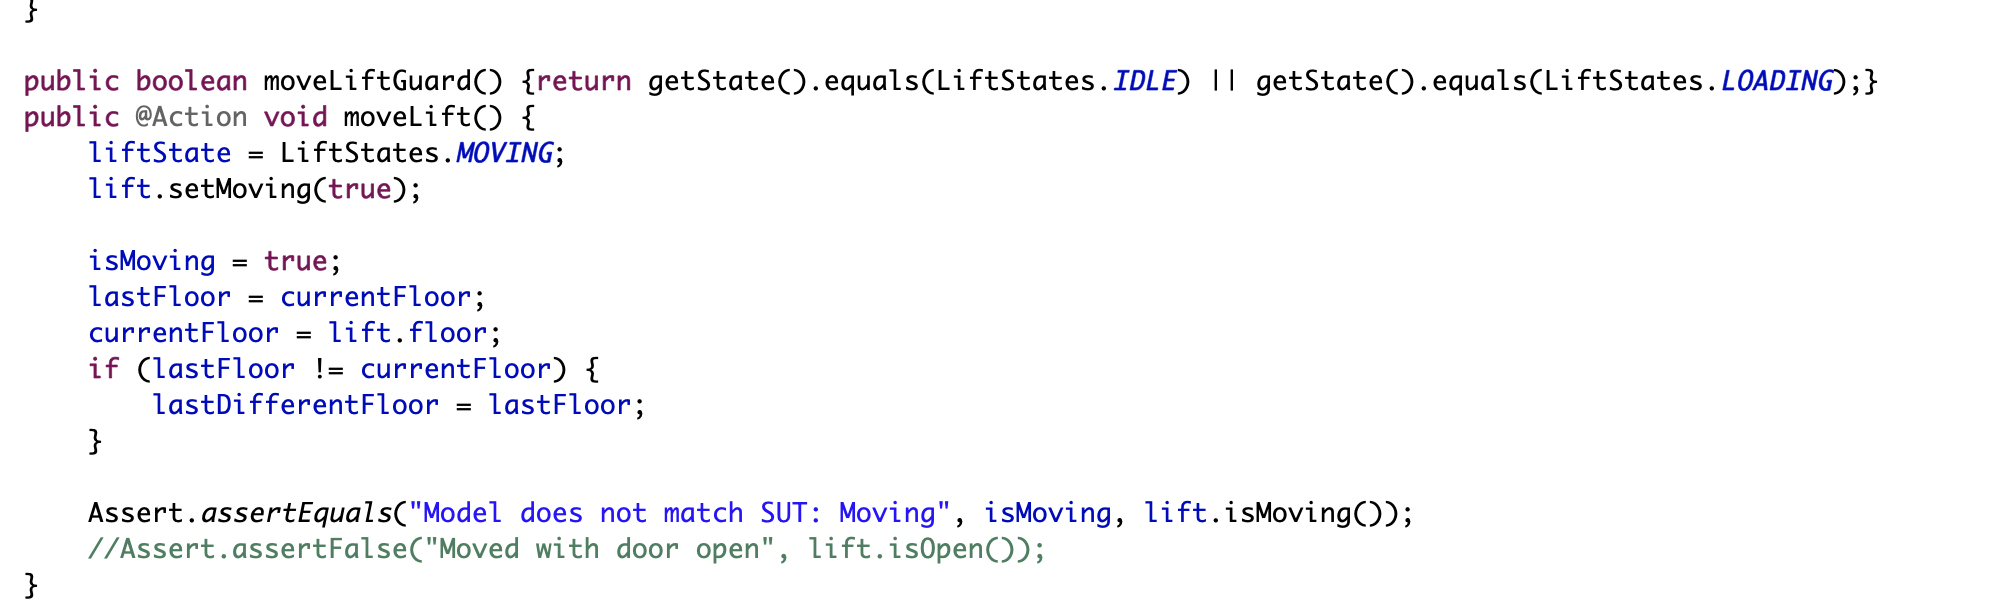
\includegraphics[width=\linewidth]{images/larva-test-fail-2-code}
  \caption{Modified code}
\end{subfigure}%
\begin{subfigure}{.5\textwidth}
  \centering
  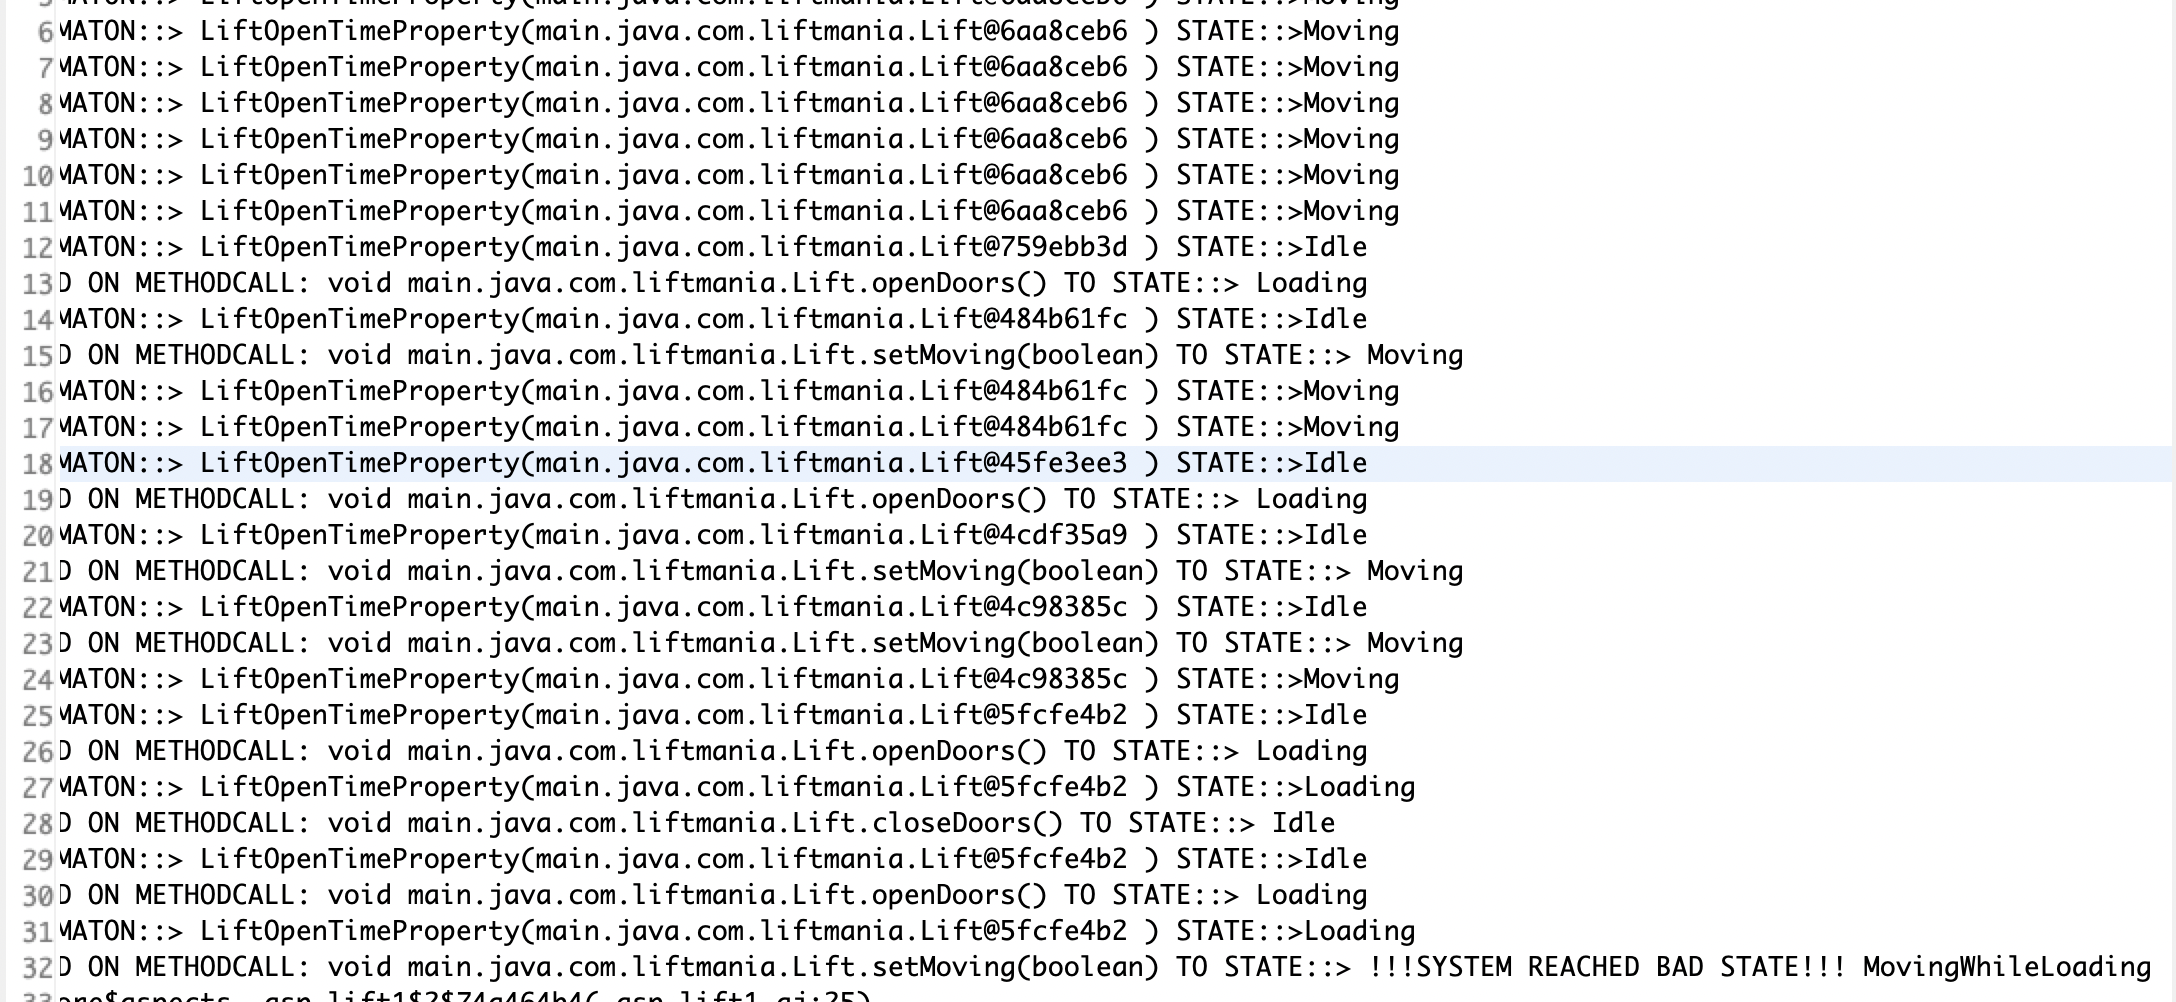
\includegraphics[width=\linewidth]{images/larva-test-fail-2-output}
  \caption{Larva output}
\end{subfigure}
\caption{RV reaches bad state from test example 2}
\label{fig:larva-test-fail-2}
\end{figure}

Overall this setup really makes sense since if one technique can better check for something than the other, when implemented together they check for all the setups. For example, checking for timed events proved to be easier in java with the help of implemented clocks. On top of that, tests help to check for all possible scenarios without having to do them manually. This means that the tests can be done unattended. Furthermore, the purpose of RV is to be deployed with systems at runtime, where real live users will be using (driving) the system instead of the programmer. Therefore, RV still needs to be implemented for the actual runtime of the system, considering that implementing RV for the model-testing was not to complicated, it would be an extremely smart and efficient move to implement the RV for the model-testing as well. \\

\end{document}
